\PassOptionsToPackage{quiet}{fontspec}
\documentclass[oneside]{ctexbook}
\usepackage{amsthm,amssymb,amsmath}
\usepackage{fancyhdr}
\usepackage{enumerate}
%\usepackage{biblatex}
\usepackage{biblatex}
\usepackage{graphicx}
\usepackage{picinpar}
\usepackage{subfig}
%\usepackage{epstopdf}
\usepackage{epsfig}
\usepackage{etoolbox}
\usepackage{showidx}
\usepackage{imakeidx}
\usepackage[colorlinks=true]{hyperref}
%tipa包用于arc命令
\usepackage{tipa}
\usepackage{listings}%排版代码的包
%\usepackage[yyyymmdd,hhmmss]{datetime}
\setlength{\headheight}{13pt}
\pagestyle{fancy}
%\rfoot{编译时间:  \today\  \currenttime}
%\cfoot{}
%\lfoot{页码:\thepage}
\newcommand{\norm}[1]{{\left | \left |  #1  \right | \right |}}
\newcommand{\inner}[2]{{\left < #1, #2 \right >}}
\newcommand{\abs}[1]{{\left | #1 \right |}}
\newcommand{\parallelsum}{{\mathbin{\!/\mkern-5mu/\!}}} %斜的平行线
\newcommand{\Hn}{{\mathbb{H}^n}}
\newcommand{\Sn}{{\mathbb{S}^n}}
\newcommand{\En}[1]{{\mathbb{R}^{#1}}}
\newcommand{\area}[1]{{\Area{#1}}}
\newcommand{\areap}{{\mathcal{A}_{+}}}
\newcommand{\arean}{{\mathcal{A}_{-}}}
\renewcommand{\div}{{\text{div}}}
\newcommand{\spt}{{\text{spt}}}
\newcommand{\tr}{{\text{tr}}}
\newcommand{\sing}{{\mathcal{S}}}
\newcommand{\proj}{{\text{Proj}}}
\newcommand{\diam}{{\text{diam}}}
\newcommand{\Tr}{{\text{Tr}}}
\newcommand{\XX}{{\vec{X}}}
\newcommand{\cl}[1]{\overline{#1}}
\newcommand{\eq}{{\equiv}}
%\newcommand{\C}{\mathbb{C}}
\newcommand{\R}{{\mathbb{R}}}
\newcommand{\nullset}{{\emptyset}}
\renewcommand{\H}{{\mathbb{H}}}
\newcommand{\N}{{\mathbb{N}}}
%\newcommand{\G}{\mathcal{G}}
\newcommand{\subsub}{{\subset \subset}}
\newcommand{\OR}{{\Omega \times \mathbb{R}}}
\newcommand{\OL}{{\Omega_L}}
\renewcommand{\epsilon}{\varepsilon}
\renewcommand{\phi}{{\varphi}}

\renewcommand{\l}{{\lambda}}
%\renewcommand{\L}{{\Lambda}}
\newcommand{\e}{{\epsilon}}
\newcommand{\E}{{\Epsilon}}
\renewcommand{\d}{{\delta}}
\newcommand{\g}{{\gamma}}
\newcommand{\G}{{\Gamma}}
\renewcommand{\a}{{\alpha}}
\newcommand{\A}{{\Alpha}}
\renewcommand{\b}{{\beta}}
\newcommand{\B}{{\Beta}}
\renewcommand{\u}{{\mu}}
%\newcommand{\U}{{\Mu}}
\renewcommand{\v}{{\nu}}
\newcommand{\V}{{\Vu}}
\newcommand{\x}{{\times}}
\renewcommand{\s}{{\quad}}
\renewcommand{\ss}{{\quad \quad}}
\newcommand{\sss}{{\quad \quad \quad}}
\renewcommand{\L}{\mathcal{L}}
\newcommand{\aij}{{a^{ij}}}
\newcommand{\dij}{{D_{ij}}}
\newcommand{\tto}[1]{{{\xrightarrow{#1}}}}
\renewcommand{\P}{{\partial}}
\newcommand{\PT}{{\partial_t}}
\newcommand{\PTF}{{\partial_t F}}
\newcommand{\PI}{{\partial_i}}
\newcommand{\PJ}{{\partial_j}}
\newcommand{\PIF}{{\partial_i F}}
\newcommand{\PJF}{{\partial_j F}}
\newcommand{\vt}{{d\mu_t}}
\newcommand{\vv}{{d\mu}}
\newcommand{\D}{{\mathbb{D}}}

\newcommand{\GG}{{\mathfrak{G}}}
\newcommand{\BR}{{B_r(x)}}
\newcommand{\GR}{{\GG \times \mathbb{R}}}
\newcommand{\EG}{{\mathfrak{E}}}
\newcommand{\HH}{{\tilde{H}}}
\newcommand{\aut}{{\text{Aut}}}
\newcommand{\AUT}{{\text{Aut}}}
\newcommand{\psl}{{\text{PSL}}}
\newcommand{\PSL}{{\text{PSL}}}
\newcommand{\mobius}{{\text{M\"obius}}}
\newcommand{\BVG}{{BV(\GG,\psi)}}
\newcommand{\BVO}{{BV(\Omega)}}
\newcommand{\PO}{{\partial \Omega}}
\newcommand{\overl}[1]{{\overline{#1}}}
\newcommand{\ol}[1]{{\overline{#1}}}
\newcommand{\oo}{{\infty}}
\renewcommand{\O}{\Omega}
\newcommand{\Poincare}{\text{Poincar\'e}}
\newcommand{\Holder}{\text{{H\"older}}}
\newcommand{\reciprocal}[1]{{\frac{1}{#1}}}
\newcommand{\rec}[1]{{\reciprocal{#1}}}
\renewcommand{\e}{\text{e}}
\newcommand{\iin}{\text{ in }}
\newcommand{\supp}{\text{supp}}
\newcommand{\osc}{\mathop{\text{osc}}}
\newcommand{\loc}{\text{loc}}
\newcommand{\SSP}[1]{{\S^+(\lambda,\Lambda,#1)}}
\newcommand{\SSN}[1]{{\S^-(\lambda,\Lambda,#1)}}
\renewcommand{\SS}[1]{{\S(\lambda,\Lambda,#1)}}
\renewcommand{\S}{\mathbb{S}}
\renewcommand{\N}{{N}}
\newcommand{\Hull}{{\text{Conv}}}
\newcommand{\MN}[1]{{\mathcal{M}^-(\lambda,\Lambda,#1)}}
\newcommand{\MP}[1]{{\mathcal{M}^+(\lambda,\Lambda,#1)}}
%\renewcommand{\iff}{\Leftrightarrow}
\renewcommand{\iff}{\Longleftrightarrow}
\newcommand{\semiholder}[1]{{[#1]}}
\newcommand{\lsc}[1]{{\text{LSC}(#1)}}
\newcommand{\usc}[1]{{\text{USC}(#1)}}
\renewcommand{\G}{\text{Graph}}
\newcommand{\CC}{{C^\infty_0}}
\newcommand{\ddt}{\frac{d}{dt}}
\newcommand{\ddtt}{\frac{d^2}{dt^2}}
\newcommand{\ddr}{\frac{d}{dr}}
\newcommand{\ppt}{\frac{\partial}{\partial_t}}
\newcommand{\Area}{\text{Area}}
\newcommand{\MM}{{\tilde{\mathcal{M}}}}
\newcommand{\M}{{\mathcal{M}}}
\newcommand{\tangent}{{\text{T}}}
\newcommand{\Laplace}{{\Delta}}
\newcommand{\T}{{\perp}}
\newcommand{\DD}{{\tilde{\nabla}}}
\newcommand{\barpartial}{{\bar{\partial}}}
\newcommand{\Haus}{{\mathcal{H}}}
\newcommand{\Res}{{\text{Res}}}
\renewcommand{\Re}{{\mathfrak{Re}}}
\renewcommand{\Im}{{\mathfrak{Im}}}
\newcommand{\II}{{\Pi}}
\newcommand{\HLaplace}{{\Delta}}
\newcommand{\CLaplace}{{\underline{\Delta}}}
\newcommand{\TS}{{\tilde{\Sigma}}}
\newcommand{\CV}{{C^\infty_0}}
\renewcommand{\CC}{{C^\infty_c}}
\newcommand{\NT}{{\nabla}}
\newcommand{\arc}[1]{{\texttoptiebar{#1}}}
\newcommand{\floor}[1]{{\lfloor {#1} \rfloor}}
\newcommand{\cycgroup}[1]{{\left< {#1} \right>}}
%\newcommand{\arc}[1]{{
%  \setbox9=\hbox{#1}%
%  \ooalign{\resizebox{\wd9}{\height}{\texttoptiebar{\phantom{A}}}\cr#1}}}

\newtheorem{theorem}{定理}[chapter]
\newtheorem*{theorem*}{定理}
\newtheorem{assumptions}{假设}
\newtheorem{lemma}[theorem]{引理}
\newtheorem{proposition}[theorem]{命题}
\newtheorem{exercise}[theorem]{习题}
\newtheorem{corollary}[theorem]{推论}
\newtheorem{definition}[theorem]{定义}
\newtheorem{question}[theorem]{问题}
\newtheorem*{question*}{问题}
\newtheorem{example}[theorem]{例}
\newtheorem*{example*}{例}
\newtheorem*{proposition*}{命题}
\theoremstyle{plain}
\newtheorem{remark}[theorem]{注}
%\newtheorem{claim}[theorem]{断言}
%\newtheorem*{claim*}{断言}

\newif\ifcomment
\def\comment{}
\def\begincomment{\ifdef{\comment}\noexpand\begingroup}
\def\endcomment{\noexpand\endgroup}

\newenvironment{subproof}[1][\proofname]{%
  \renewcommand{\qedsymbol}{$\diamond$}%
  \begin{proof}[#1]%
}{%
  \end{proof}%
}

\usepackage{enumitem,xparse}
\newlist{Claim}{description}{2}
\setlist[Claim]{labelindent=2em, leftmargin=*}
\newif\ifInsideClaim
\newcounter{claim}[theorem]
%\newcounter{cclaim}[claim]
\renewcommand\theclaim{\arabic{claim}}
%\renewcommand\thecclaim{\arabic{claim}.\arabic{cclaim}}
\let\originalqedsymbol\qedsymbol
\newenvironment{claim}{%
	% disable qed symbol if there is no star
	%\let\qedsymbol\relax%
	%\let\qedsymbol$\diamond$
	%\ifInsideClaim% we have a nested environment
	%\refstepcounter{cclaim}%
	%\let\theclaimcounter\thecclaim%
	%\else%
	\refstepcounter{claim}%
	\let\theclaimcounter\theclaim%
	%\InsideClaimtrue%
	%\fi%
	\Claim\item[\textbf{断言 \theclaimcounter:}]%
}{\endClaim\InsideClaimfalse\let\qedsymbol\originalqedsymbol}



\DeclareSourcemap{
  \maps[datatype=bibtex]{
    \map{
       \step[fieldset=URL, null]
       \step[fieldset=DOI, null]
       \step[fieldset=MRREVIERER, null]
       \step[fieldset=ISBN, null]
       \step[fieldset=ISSN, null]
       \step[fieldset=SERIES, null]
    }
  }
}

%\renewcommand\appendix{\par
%    \setcounter{section}{0}
%    \setcounter{subsection}{0}
%    \gdef\thesection{附录 \Alph{section}}}
%
\addbibresource{minisurf.bib}

\newif\ifshow
%\showtrue % comment out to hide answers

\newif\ifsee
\seetrue

\fancyfoot[RO]{\today}
%\fancyfoot[LE]{\today}

%\defbibheading{bibliography}[参考文献]{\chapter*{#1}}
\begin{document}
\title{课程:极小曲面}
%\author{主讲:高强}
\author{draft version}
\date{修改日期: {\today}}
%\date{2022年秋季学期}
\maketitle
\tableofcontents
\input{Chapter01}
\chapter{曲率估计}
\section{逐点估计}
设$\Sigma^{n-1} \subset \M^n$是光滑子流形. $\vec{n}$是 $\Sigma$的单位法向. 设$T$是$(0,2)$型张量, $T=T_{ij}dx^idx^j$. 记号约定如下.
\begin{equation}
    (\nabla^2_{XY}T)(Z,W)=\nabla^2T(Z,W,Y,X).
\end{equation}
在局部坐标下,
\begin{equation}
    \nabla^2_{lk}T_{ij}=(\nabla^2_{\partial l,\partial k}T)(\PI,\PJ)=\nabla^2T(\PI,\PJ, \partial k,\partial l)=T_{ijkl}.
\end{equation}
Codazzi方程.
\begin{equation}
    R^\M(X,Y,W,\vec{n}) = \nabla \II(W,Y,X) - \nabla \II (W,X,Y).
\end{equation}
Gauss方程
\begin{equation}
    R^\M(X,Y,Z,W) = R^\Sigma(X,Y,Z,W)-\II(X,W)\II(Y,Z)+\II(X,Z)\II(Y,W).
\end{equation}
求导交换次序.
\begin{equation}
    \nabla^2_{X,Y}T(Z,W) = \nabla^2_{Y,X}T(Z,W)-T(R(X,Y)Z,W)-T(Z,R(X,Y)W).
\end{equation}
在局部坐标下,
\begin{equation}
    T_{ijkl}=T_{ijlk}-R_{lki}^pT_{pj}-R_{lkj}^pT_{ip}.
\end{equation}
求导交换次序的结果可以参考\cite[定理7.14]{lee}. 需要注意, $T_{ijkl}=(\nabla^2_{lk}T)(\PI,\PJ)$.  
\begin{proposition}
    设$\Sigma^{n-1} \subset \R^n$是光滑曲面. $\nabla, \Delta$为$\Sigma$上的算子. $\II$为其第二基本型, $H$是平均曲率. 则
    \begin{equation} \label{simon1}
        \Delta \II_{ij}=\nabla^2_{ij}H + Hg^{kl}\II_{ik}\II_{jl}-\abs{\II}^2\II_{ij}.
    \end{equation}
\end{proposition}
\begin{proof}
    固定点$p$, 选取$p$点附近的测地坐标, 则有
    \begin{equation}
        \Delta \II_{ij}=\II_{ij;kk}=\II_{ik;jk}=\II_{ik;kj}-R_{kji}^p\II_{pk}-R_{kjk}^p\II_{ip}.
    \end{equation}
    而
    \begin{equation}
        \II_{ik;kj}=\II_{kk;ij}=H_{ij}.
    \end{equation}
    \begin{equation}
        \begin{split}
            R_{kji}^p\II_{pk}+R_{kjk}^p\II_{ip} &= R_{kjip}\II_{pk}+R_{kjkp}\II_{ip}\\
            &=\II_{kp}\II_{ji}\II_{kp}-\II_{ki}\II_{jp}\II_{pk}+\II_{kp}\II_{jk}\II_{ip}-\II_{kk}\II_{jp}\II_{ip} \\
            &=\abs{\II}^2\II_{ij}-Hg^{pq}\II_{jp}\II_{iq}
        \end{split}
    \end{equation}
\end{proof}
\begin{proposition}[Simons等式] \label{simon_equation}
    设$\Sigma^{n-1}$是极小曲面, 则有
    \begin{equation}
        \Delta\abs{\II}^2 = 2(\abs{\nabla \II}^2-\abs{\II}^4).
    \end{equation}
\end{proposition}
\begin{proof}
    将等式\eqref{simon1}写成坐标无关的形式, 又因$\Sigma$是极小曲面, 则有
    \begin{equation}
        \Delta \II = -\abs{\II}^2 \II
    \end{equation}
    由于$\Tr$与联络导数可交换, 则
    \begin{equation}
        \begin{split}
            \Delta \abs{\II}^2 = \Delta (\Tr^2(\II\otimes\II)) &= \Tr^2(\Delta \II \otimes\II + \II \otimes \Delta \II + 2 \Tr(\nabla \II, \nabla \II)) \\
            &=\Tr^2(-2\abs{\II}^2 \II\otimes\II+2\Tr(\nabla \II \otimes \nabla \II)) \\
            &=-2\abs{\II}^4+2\abs{\nabla \II}^2.
        \end{split}
    \end{equation}
\end{proof}
\begin{proposition}[Simons不等式]
    设$\Sigma^{n-1}$是极小曲面, $\nabla,\Delta$为$\Sigma$上的算子. 则
    \begin{equation} \label{simon_inequality}
        \Delta \abs{\II}^2 \ge -2\abs{\II}^4+2(1+\frac{2}{n-1})\abs{\nabla \abs{\II}}^2.
    \end{equation}
\end{proposition}
\begin{proof}
    证明与命题\eqref{kato}类似. 我们首先来计算 $\abs{\nabla \abs{\II}}^2$. 固定点$p$, 取$p$点处的测地坐标使得$\II=diag(\lambda_i)$.
    \begin{equation} \label{s11}
        \begin{split}
            \abs{\nabla \abs{\II}}^2 = \frac{\abs{\inner{\nabla \II}{\II}}^2}{\abs{\II}} &= \frac{\sum_j(\sum_i\lambda_i\II_{iij})^2}{\sum_i\lambda_i^2} \\
            &\le \sum_{ji}\II_{iij}^2
        \end{split}
    \end{equation}
    而
    \begin{equation} \label{s12}
        \begin{split}
            \sum_{ji}\II_{iij}^2 &= \sum_{j\ne i}\II_{iij}^2+ \sum_{i}\II_{iii}^2 \\
            &= \sum_{j\ne i}\II_{iij}^2+ \sum_{i}(-\sum^{n-1}_{j \ne i}\II_{jji})^2\\
            &\le \sum_{j\ne i}\II_{iij}^2+ \sum_{i}(n-2)\sum_{j\ne i}\II_{jji}^2\\
            &\le (n-1)\sum_{j\ne i}\II_{iij}^2\\
            &= \frac{n-1}{2}(\sum_{j\ne i}\II_{iji}^2 +\sum_{j\ne i}\II_{jii}^2)
        \end{split}
    \end{equation}
    \eqref{s12}两侧同乘以$\frac{2}{n-1}$后与\eqref{s11}相加可得,
    \begin{equation}
        \begin{split}
            \abs{\nabla \abs{\II}}^2+\frac{2}{n-1} \abs{\nabla \abs{\II}}^2 &\le \sum_{ji}\II_{iij}^2 + \sum_{j\ne i}\II_{iji}^2 +\sum_{j\ne i}\II_{jii}^2 \\
            &\le \sum_{ijk}\II^2_{ijk}
        \end{split}
    \end{equation}
    再由Simon等式\eqref{simon_equation}即可得到不等式\eqref{simon_inequality}.
\end{proof}
\begin{theorem}\label{choi_schoen}
    设$\Sigma^2 \subset \R^3$是极小曲面.  则存在常数$\epsilon, \rho>0$, 使得 $\forall p \in \Sigma, r_0 < \rho$, 如果
    \begin{enumerate}
        \item $\partial \Sigma \cap B_{r_0}(p)=\emptyset$.
        \item $\int_{\Sigma \cap B_{r_0}} \abs{\II}^2\le \epsilon$.
    \end{enumerate}
    那么$\forall  0 < \sigma \le r_0$及$y \in B_{r_0-\sigma}$, 成立
    \begin{equation}
        \sigma^2 \abs{\II}^2(y) \le \delta, \text{ here }\delta= \frac{\int_{\Sigma \cap B_{r_0}}\abs{\II}^2}{\epsilon}.
    \end{equation}
\end{theorem}
\begin{proof}
    将$B_{r_0}$简写为$B$. 只需要证明$F(x)=d^2(x,\P B)\abs{\II}^2(x) \le \delta$即可. 我们用反证法. 设$F$在$q$点处取到最大值$\max_{x \in B}F(x)$. 注意到在$\partial B$上, $F(x) \eq 0$. 则$q$是内点.  设$F(q) > \delta$, 我们将证明当$\epsilon$足够小时, 会推出一个矛盾. 取 $\sigma$使得
    \begin{equation}
        \sigma^2\abs{\II}^2(q)=\frac{\delta}{4} \le \frac{1}{4} d^2(q,\P B)\abs{\II}^2(q).
    \end{equation}
    因此, 有
    \begin{equation}
        \sigma \le \frac{1}{2}d(q,\P B).
    \end{equation}
    由三角不等式可知,  $\forall y \in B_\sigma(q)$,
    \begin{equation}
        \frac{1}{2} \le \frac{d(y,\P B)}{d(q,\P B)} \le 2.
    \end{equation}
    于是
    \begin{equation}
        \begin{split}
            \sup_{y\in B_\sigma(q)} d^2(q,\P B) \abs{\II}^2(y) \le &4\sup_{y\in B_\sigma(q)}d^2(y,\P B)\abs{\II}^2(y) \\
            =& 4d^2(q,\P B) \abs{\II}^2(q).
        \end{split}
    \end{equation}
    因此,
    \begin{equation}
        \sup_{y \in B_\sigma(q)} \abs{\II}^2(y) \le 4\abs{\II}^2(q)=\frac{\delta}{\sigma^2}.
    \end{equation}
    通过变换$x\to \sigma x$, 上面的不等式变为
    \begin{equation} \label{ii_sup}
        \sup_{y \in B_1(q)} \abs{\II}^2(y) \le 4\abs{\II}^2(q)=\delta \le 1.
    \end{equation}
    由Simons不等式, 我们得到
    \begin{equation}
        \Delta \abs{\II}^2 \ge -2\abs{\II}^4 \ge -2 \abs{\II}^2.
    \end{equation}
    由推论\eqref{sub_harmonic}(取$s=1,\lambda=2$)可知,
    \begin{equation}
        \frac{\delta}{4}=\abs{\II}^2(q) \le C \int_{B_1} \abs{\II}^2 \le C\delta\epsilon.
    \end{equation}
    则当$\epsilon$足够小时, 显然是不可能的.
\end{proof}
把定理\eqref{choi_schoen}写成下面形式往往是方便的.
\begin{theorem*}\label{choi_schoen_cor}
    设$\Sigma^2 \subset \R^3$是极小曲面.  则存在常数$\epsilon, \rho>0$, 使得 $\forall r_0 < \rho$, 如果
    \begin{enumerate}
        \item $\partial \Sigma \cap B_{r_0}(p)=\emptyset$.
        \item $\int_{\Sigma \cap B_{r_0}} \abs{\II}^2\le \epsilon$.
    \end{enumerate}
    那么
    \begin{equation}
        \mathop{\sup}_{B_{\frac{r_0}{2}}}\abs{\II(x)} \le \frac{C}{r_0}.
    \end{equation}
\end{theorem*}

\begin{lemma}[一致图像引理] \label{uniform_graph}
    设$\Omega \subset \R^3$是具有光滑边界的开集. 设$\Sigma^2 \subset \Omega$是嵌入的光滑曲面, 并且$\Sigma$在$\Omega$中是闭的. 设$\abs{\II} \le C$. 则$\Sigma$可以局部一致地表示成函数图像的形式. 确切地说, $\forall p \in \Sigma$, $R\in (0,R_0)$. 这里, 
    \begin{equation}
        R_0=\min\{\frac{1}{4C}, \frac{1}{2}d(p,\partial \Omega)\}.
    \end{equation}
    设$D(p,R)$为$T_p\Sigma$上以$p$为中心, 半径为$R$ 圆盘, $W(p,R)=D(p,R)\times \R$. 
    \begin{align}
        &D(p,R)= \{p+\vec{v}\mid v \in T_p\Sigma, \abs{v} < R\}.  \\
        &W(p,R)= \{q+t\vec{n}(p)\mid q \in D(p,R), t \in \R\}.
    \end{align}
    则存在函数$u: D(p,R)\to \R$ 使得$u(p)=0$, 并且$\Sigma$可以写成$u$的在$D(p,R)$上的图像的形式. 并且, 给定$q \in D(p,R)$,
    \begin{enumerate}
        \item $\abs{u(p)-u(q)} \le 8C\abs{p-q}$.
        \item $\abs{\nabla u}(q) \le 8C\abs{p-q}$.
        \item $\abs{\nabla^2 u}(q) \le 16C$.
    \end{enumerate}
\end{lemma}
\begin{remark}
    一致图像引理不要求曲面是极小的.
\end{remark}
\begin{proof}
    设$\Sigma_{p,r}$是$\Sigma \cap W(p,r)$的包含$p$点的连通分支.  经过旋转平移之后, 设$p =0, T_p\Sigma = \{z=0\}$. 设$R \in \R$满足以下条件, 并且取上界: $\Sigma_{p,R}$可以表示为某个函数$u \in C^\infty(D(p,R))$的图像, $u(0)=0, \nabla u(p)=0$ 且 $\abs{\nabla u} \le 1$. 注意, $\abs{\nabla u} \le 1$等价于$N_3=\inner{\vec{n}}{e_3}=\frac{1}{\sqrt{1+\abs{Du}^2}} \ge \frac{1}{2}$. 现在, 当$R$变得更大一点时, 有两种情况可能发生:
    \begin{enumerate}
        \item 函数$u$可以光滑地延拓到$D(p,R)$的邻域内, 但是会导致$N_3< \frac{1}{2}$. \label{case1}
        \item 函数$u$不能继续延拓, 这表明$\G(u)$碰到了$\Omega$的边界. \label{case2}
    \end{enumerate}
    直接计算可知, 我们有如下的比较关系
    \begin{equation}
        \frac{\abs{\nabla^2 u}^2}{(1+\abs{\nabla u}^2)^3} \le \abs{\II}^2 \le 2 \frac{\abs{\nabla^2 u}^2}{1+\abs{\nabla u}^2}.
    \end{equation}
    在$D(p,R)$上, 由于$\abs{Du} \le 1$, 则
    \begin{equation}
        C^2 \le \abs{\nabla^2 u} \le 8C^2.
    \end{equation}
    现在, 设情况\eqref{case1}发生, 设$q \in \partial D(p,R)$使得$\abs{\nabla u(q)}=\frac{1}{2}$. 则
    \begin{equation}
        1=\abs{\nabla u(0)-\nabla u(q)} \le \abs{\nabla^2 u}\abs{q}\le 4CR.
    \end{equation}
    因此, $R \ge \frac{1}{4C}$.
    若情况\eqref{case2}发生,  设$Q=(q,u(q))\in \partial \Omega, q \in \partial D(p,R)$. 设$\alpha$是连接 $p,q$的线段, 则
    \begin{equation}
        d(p,Q) \le \sup \sqrt{1+\abs{\nabla u}}l_\alpha \le 2R.
    \end{equation}
    即有$R \ge \frac{1}{2}{d(p,\partial \Omega)}$.  其余性质均可由中值定理得到.
\end{proof}
\begin{corollary} \label{choi_schoen_intrinsic}
    定理\eqref{choi_schoen}中的$B_r$可以换成$B^\Sigma_r$.
\end{corollary}
\begin{proof}
    在定理\eqref{choi_schoen}的证明中, 有了不等式\eqref{ii_sup}(欧氏度量换成内蕴度量后, 直到这里的推导都是正确的), 我们就可以用应用一致图像引理. 由于此时$\abs{\nabla u}$一致有界, 那么$\Sigma$上的内蕴度量与外蕴度量实际上是局部可比较的. 最后在$B_\frac{1}{4}$(引理\eqref{uniform_graph}中, $C=1$)上应用推论\eqref{sub_harmonic}.
\end{proof}

\begin{theorem} \label{compactness}
    设$\{\Sigma_i \} \subset \R^3$是完备极小曲面. 设$p_i \in \Sigma_i$且$p_i \to p$.  设存在常数$C$使得$\forall i$,
    \begin{equation}
        \abs{\II_{\Sigma_i}} \le C.
    \end{equation}
    则存在子列$\Sigma_{i_k}$及极小曲面$\Sigma$使得$\Sigma_{i_k} \overset{C^\infty}{\longrightarrow} \Sigma$.
\end{theorem}
\begin{proof}
    在$p$点处, (选取子列)设$T_{p_k}\Sigma_k \to \{z=0\}$.  设$B_\delta(0)=\{(x,y,z)\mid z=0, x^2+y^2 \le \delta^2\}$. 由一致图像引理, 存在$\delta=\delta(C)>0$使得$\Sigma_k$可以表示成为$B_\delta(0)$上的函数$u_k$的图像, 且在$B_\delta$上, $Du_k$一致有界. 则存在函数$u$使得 $u_k \to u$. 由Schauder估计可知, $u_k \overset{C^\infty}{\longrightarrow} u$.  
    \par 取$p \in \P B_\delta(0)$, 则在$p$点的$\delta$邻域中,  重复上面的过程. 我们可以得到在更大区域上的收敛子列.  此过程可以一直继续下去, 直到我们得到完备的极小曲面.
\end{proof}
在后面的曲率估计中, 下面的引理将会被频繁用到.
\begin{lemma}
    设$\Sigma \subset \R^3$是嵌入的光滑曲面. 则
    \begin{equation}
        d(x,\P \Sigma)\abs{\II(x)},\s  \int_\Sigma \abs{\II}^2dv_g
    \end{equation}
    是在伸缩变换下的不变量.
\end{lemma}
\begin{theorem}
    存在常数$C>0$使得对于任意定向的稳定极小曲面$\Sigma^2 \subset \R^3$, 成立
    \begin{equation}
        d_\Sigma(x,\P \Sigma)\abs{\II}(x)  \le C.
    \end{equation}
\end{theorem}
\begin{proof}
    反证法. 设存在稳定极小曲面$\Sigma_k$及$p_k \in \Sigma_k$使得
    \begin{equation}
        d(p_k, \P \Sigma_k)\abs{\II_k(p_k)}  \to \infty.
    \end{equation}
    如果$\Sigma_k$是无界的, 则截断$\Sigma_k$使其是带有光滑边界的紧集. 不失一般性, 设$p_k$取到$d(x,\P \Sigma_k)\abs{\II_k(x)}$的最大值. 经过平移旋转后, 设 $p_k$在0点处. 对$\Sigma_k$做伸缩变换$ x \to \abs{\II_k(p_k)}x$, 得到新的极小曲面列, 仍记为 $\Sigma_k$. 这些新的极小曲面仍然满足: $\Sigma_k$是稳定的, 并且$d(0, \P \Sigma_k)\abs{\II_k(0)} \to \infty$. 另外,  $\abs{\II_k(0)}=1$. 因此, $d(0, \P \Sigma_k) \to \infty$. 根据$p_k$的选取, $\forall x \in \Sigma_k$,
    \begin{equation}
        d(x,\P \Sigma_k)\abs{\II_k(x)} \le d(0,\P \Sigma_k).
    \end{equation}
    设$x \in B_r$. 则
    \begin{equation}
        \abs{\II_k(x)} \le \frac{d(0,\P \Sigma_k)}{d(x,\P \Sigma_k)} \to 1.
    \end{equation}
    因此, $\abs{\II_k}$局部一致有界. 根据定理\eqref{compactness}, 存在极小曲面$\Sigma$使得$\Sigma_k \overset{C^\infty}{\longrightarrow} \Sigma$. 显然$\Sigma$是完备的, 且$\abs{\II(0)}=1$. 下面我们说明$\Sigma$是稳定的.  否则的话, 存在$\Omega \subsub \Sigma$使得$\lambda_1(\L_\Sigma,\Omega) < 0$. 而由于$\Sigma_k \overset{C^\infty}{\longrightarrow} \Sigma$, $\L_{\Sigma_k} \to \L_\Sigma$, 则$\Sigma$是稳定的. 而由定理\eqref{stable_flat}可知, $\Sigma$是平面, 而这与$\abs{\II(0)}=1$矛盾.
\end{proof}
%\begin{proof}
%    记$r_0=d(x,\partial \Sigma)$. 由命题\eqref{mc_area}可知, $\forall 0<r < r_0$, 
%    \begin{equation}
%        \Area(B^\Sigma_r) \le Cr^2.
%    \end{equation}
%    (这里如果$B^\Sigma_r$不是嵌入圆盘, 我们就在万有覆盖中来做). 固定$x$, 设$r=d(y,x)$, 定义截断函数
%    \begin{equation}
%        \eta(y)=\left\{
%            \begin{aligned}
%                & 1, r\le e^{-N}r_0, \\
%                & \frac{\log r_0-\log r}{N}, e^{-N}r_0 < r < r_0, \\
%                & 0, r>r_0.
%            \end{aligned}
%        \right.
%    \end{equation}
%    由于$\abs{\nabla r}=1$, 则$\abs{\nabla \eta} \le \frac{1}{Nr}$. 将$\eta$代入到稳定性不等式中, 得到
%    \begin{equation}
%        \begin{split}
%            \int_{B^\Sigma_{e^-Nr_0}}\abs{\II}^2 \le \int_\Sigma \eta^2 \abs{\II}^2 &\le \int_\Sigma \abs{\nabla \eta}^2  \\
%            &\le \frac{1}{N^2}\sum_{i=-n}^{-1}\int_{B_{e^{i+1}r_0}^\Sigma-B_{e^ir_0}^\Sigma}\frac{1}{r^2} \\
%            &\le \frac{4\pi e^2}{3N}.
%        \end{split}
%    \end{equation}
%    $N$取足够大时就可以应用定理\eqref{choi_schoen}(推论\eqref{choi_schoen_intrinsic}).
%\end{proof}
\begin{theorem} \label{curvature_estimate_4pi}
    设$C \in (0,8\pi)$. 则存在常数$C_0=C_0(C)$使得: 如果$\Sigma \subset \R^3$是定向极小曲面, 并且
    \begin{equation}
        \int_\Sigma \abs{\II}^2 dv_g \le C.
    \end{equation}
    则$\forall x \in \Sigma$,
    \begin{equation}
        d(x,\P \Sigma)\abs{\II(x)} \le C_0.
    \end{equation}
\end{theorem}
定理\eqref{curvature_estimate_4pi}的证明需要下面的定理\eqref{total_curvature}.
\begin{theorem}\label{total_curvature}
    设$\Sigma^2$是非紧, 可定向, 完备的2维黎曼流形, 并且
    \begin{equation}
        \int_\Sigma K^- < +\infty. 
    \end{equation}
    这里, $K^-=-\min(K,0)$, $K$是Gauss曲率. 则有
    \begin{enumerate}
        \item $\int_\Sigma \abs{K} dv_g < +\infty$.
        \item 存在闭黎曼面$\mathcal{S}$及$\{p_1,p_2\cdots p_k\} \subset \mathcal{S}$使得$\Sigma$共形同构于$\mathcal{S}-\{p_i\}$.
    \end{enumerate}
    如果$\Sigma \subset \R^3$是极小曲面, 则
    \begin{enumerate}
        \item[3.] 存在$m \le 0$使得 $\int_\Sigma K dv_g = 4m\pi$.
    \end{enumerate}
\end{theorem}
\begin{proof}
    设$p \in \Sigma$. 记$D_r=D(p,r)=\{x\in \Sigma \mid d_\Sigma(p,x) \le r\}$, 则$\P D_r$是分段光滑曲线. 设$\{\theta^r_i\}$是$\P D$上的非光滑点处的外角, 如是图所示.
    \begin{figure}[ht]
        \centering
        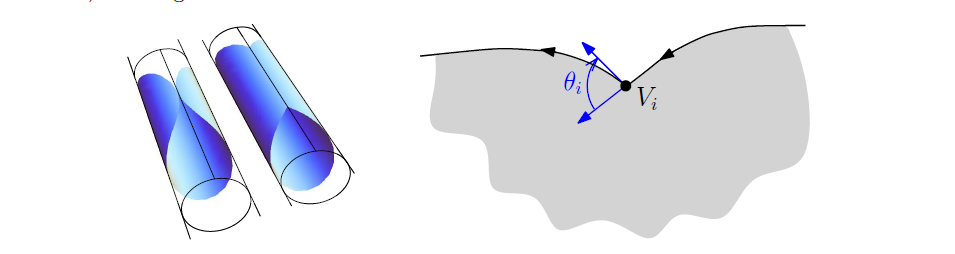
\includegraphics[scale=0.8]{images/angle.png}
        \caption{区域$D_r$的边界.}
        \label{angle}
    \end{figure}
    我们这里选取的定向使得$-\pi \le \theta_i \le 0$.  记$l(r)=l(\P D_r)$. 则由第一变分公式(非光滑点附近需要单独处理, 参考\cite{White}及\cite{Perez}),
    \begin{equation}
        l'(r)=\int_{\P D_r}K_{\P D}ds+2\sum \tan(\frac{\theta_i}{2}).
    \end{equation}
    而由于$\tan(\frac{\theta_i}{2}) \le \frac{\theta_i}{2}$, 及Gauss-Bonnet公式(分段光滑区域上的Gauss-Bonnet公式参考\cite{lee}),
    \begin{equation}
        l'(r)\le \int_{\P D_r}K_{\P D}ds+\sum \theta_i = 2\pi\chi(D_r)-\int_{D_r}Kdv_g.
    \end{equation}
    由于$\mathop{\limsup} l'(r) \ge 0$(若$ \mathop{\limsup l'(r)} \le \alpha <0$, 则存在$r$足够大使得$l(r) < 0$, 这是不可能的), 则有
    \begin{equation} \label{basic_inequality}
        \begin{split}
            0 &\le \limsup_{r\to \infty} l'(r) \le \limsup(2\pi \chi(D_r) - \int_{D_r}Kdv_g) \\
            & \le \limsup (2\pi(2-2p(D_r)-(\P D_r)^\#)-\int_{D_r}K^+dv_g+\int_{D_r}K^-dv_g)
        \end{split}
    \end{equation}
    其中, $p$为$D_r$的亏格, $(\P D_r)^\#$为$D_r$的边界的连通分支数. 上述不等式意味着, 存在常数$C$使得
    \begin{enumerate}
        \item $p(D_r), (\P D_r)^\#, \int_{D_r}K^+dv_g \le C(\int_\Sigma K^-dv_g +1)$. \label{finite}
        \item 存在$r_0>0$使得$\forall r > r_0$, $p(D_r) = p(D_{r_0})$. \label{genus}
    \end{enumerate}
    结论\eqref{finite}由\eqref{basic_inequality}取极限直接得到. 结论\eqref{genus}是因为$p(D_r)$是有上界的, 且$p(D_r)$只取整数值且关于$r$是非减的. 现在, 对于$\Sigma - D_r$,我们证明
    \begin{claim}
        设$r > r_0$, 则$\Sigma - D_r$的每一个紧的连通分支都是单连通的.
        \begin{subproof}
            设$\Omega$是$\Sigma - D_r$的一个连通分支. 若$\P \Omega$至少包含两个边界, 由于$\P \Omega \subset \P D_r$, 则$p(D_r \cup \Omega) > p(D_r)$, 这与结论\eqref{genus}矛盾. 断言证毕.
        \end{subproof}
    \end{claim}
    \par 现在, 记$A_r=D_r\cup \{\Sigma - D_r\text{的所有紧连通分支}\}$. 同时取$r_i$使得\eqref{basic_inequality}成立并且
    \begin{equation} \label{boundary_constant}
        (\P D_{r_i})^\# = (\P D_{r_{i+1}})^\#=c.
    \end{equation}
    $(\P D_{r})^\#$总是取整数值并且有上界, \eqref{boundary_constant}是可以取到的. 由于$(\P A_{r_i})^\# \le (\P D_{r_i})^\#$, 可设
    \begin{equation}
        (\P A_{r_i})^\# = (\P A_{r_{i+1}})^\#=c'.
    \end{equation}
    此时, $A_{r_i} \subset A_{r_{i+1}}$并且 $A_{r_i}$与$A_{r_{i+1}}$同胚, 则$A_{r_{i+1}}$是由$A_{r_i}$在边界处添加annulus而得到. 由于$\Sigma = \cup A_{r_i}$, 则$\Sigma$与 $A_{r_i}$具有相同的拓扑型. 现在可以在不等式\eqref{basic_inequality}可以得到,
    \begin{equation}
        \begin{split}
            0 & \le \limsup (2\pi(2-2p(D_r)-(\P D_r)^\#)-\int_{D_r}K^+dv_g+\int_{D_r}K^-dv_g) \\
            &\le  \limsup (2\pi(2-2p(A_r)-(\P A_r)^\#)-\int_{A_r}Kdv_g) \\
            & \to  2\pi \chi(\Sigma) - \int_\Sigma K dv_g.
        \end{split}
    \end{equation}
    至此, 我们已经证明了$\Sigma$是有限型曲面, 即同胚于闭区曲面去掉有限个点.
    \par 设$E$为$\Sigma$的一个末端 (end, 即$\Sigma-D_{r_0}$的一个连通分支, $r_0$取足够大). 则$E$是annulus. 
    \begin{claim}
        $E$共形同构于$\{1 < \abs{z} < +\infty\}$.
        \begin{subproof}
            记$\Gamma_r=\P D_r \cap E$. 设$\phi: E \to \{ 1 < \abs{z} < R\}$是共形等价. 我们需要证明$R=+\infty$. 设$\Gamma_r(s)$是其弧长参数化. 则
            \begin{equation}
                2\pi = l_{\S^1} \le l_{\phi\circ \Gamma_r} = \int_{\Gamma_r} \abs{d \phi(\Gamma_r)\Gamma'_r}ds.
            \end{equation}
            由Cauchy不等式, 则有
            \begin{equation}
                \begin{split}
                    4\pi^2 \le (\int_{\Gamma_r} \abs{d\phi(\Gamma_r)\Gamma'_r}ds)^2 & \le l_{\Gamma_r}\int_{\Gamma_r}\abs{D\phi(\Gamma_r)}^2ds \\
                    & =l(\Gamma_r)\int_{\Gamma_r}\det \phi ds.
                \end{split}
            \end{equation}
            (最后一个等式中, 我们用到了对于全纯函数$\phi$, $\abs{d\phi}^2 = \abs{\phi'}^2= \det \phi$). 由于
            \begin{equation}
                l'(r) \le 2\pi\chi(D_r) - \int_{D_r}Kdv_g \to 2\pi\chi(\Sigma) - \int_\Sigma K dv_g,
            \end{equation}
            则存在常数$C$使得 
            \begin{equation}
                l(r) \le Cr.
            \end{equation}
            综合以上几个不等式, 我们得到
            \begin{equation}
                \frac{4\pi^2}{Cr} \le \frac{4\pi^2}{l(r)} \le \frac{4\pi^2}{l_{\Gamma_r}} \le \int_{\Gamma_r}\det\phi ds.
            \end{equation}
            对$r$积分, 则有
            \begin{equation}
                \begin{split}
                    +\infty = \int^\infty_{r_0} \frac{4\pi^2}{Cr} &\le \int^\infty_{r_0}\int_{\Gamma_r} \det\phi dsdr  \\
                    &=\Area(\phi(E)) \\
                    &= \Area(\{1<\abs{z}< R\}) 
                \end{split}
            \end{equation}
            因此, $R=+\infty$, 断言证毕.
        \end{subproof}
    \end{claim}
    现在设$\Sigma$是极小曲面, 我们计算$\Sigma$的全曲率.  由命题\eqref{pullback_gauss}可知,
    \begin{equation}
        \int_\Sigma K dv_g = - \Area(N(\Sigma)).
    \end{equation}
    $N$为Gauss映射. 等式右侧面积的计算需要计象集中每个点的重数. 现在, 我们需要说明存在一个整数重数. 
    \begin{claim}
        设$\Sigma$共形等价于$\mathcal{S}-\{p_i\}$, $\mathcal{S}$是闭黎曼曲面.  则其Gauss映射$g: \Sigma\to \overline{\mathbb{C}}$可以延拓为$\mathcal{S}$上的亚纯函数.
        \begin{subproof}
            取$p \in \{p_i\}$, 并取$p$点的邻域, 设这个领域共形等价于$\D^*=\D - \{0\}$. 现在, 可以将$g$看作$g: \D^* \to \overline{\mathbb{C}}$. 设$\gamma_\rho=\{\abs{z}=\rho\}$, 并取$\gamma_\rho$的弧长参数化. 则有
            \begin{equation}
                \abs{l_{g(\gamma_\rho)}}^2 = (\int_{\gamma_\rho} \abs{dg(\gamma_\rho) \gamma'_\rho(s) ds})^2 \le 2\pi\rho \int_{\gamma_\rho}\abs{dg(\gamma_\rho)}^2ds.
            \end{equation}
            两侧同时除以$\frac{1}{2\pi\rho}$并对$\rho$积分, 则有
            \begin{equation}
                \begin{split}
                    \int^1_0 \frac{l^2(g(\gamma_\rho))}{2\pi\rho} d\rho \le \int^1_0 \int_{\gamma_\rho} \abs{dg(\gamma_\rho)}^2dsd\rho &= 2\Area(g(\D^*))  \\
                    &\le -2\int_\Sigma Kdv_g<\infty.
                \end{split}
            \end{equation}
            最后一个不等式是因为命题\eqref{pullback_gauss}. 由于$\frac{1}{\rho}$不可积, 则存在$\rho_i \to 0$使得  $l(g(\rho_i)) \to 0$. 这意味着$g$在0点的邻域内有界. 因此, $g$可以延拓为$\mathbb{D}$上的亚纯函数. 断言得证.
        \end{subproof}
    \end{claim}
    \par  由于黎曼面之间的共形映射是覆盖映射(除去有限个分歧点), 则
    \begin{equation}\label{total_curvature_degree}
        \int_\Sigma Kdv_g = - \text{deg}(g) \Area(\S^2) = -\text{deg}(g)4\pi.
    \end{equation}
\end{proof}
\begin{remark}
    上面等式\eqref{total_curvature_degree}实际上提供了一种计算完备极小曲面全曲率的方法: 只需要知道Gauss映射下$\S^2$上任意一个点的原像的个数, 乘以$4\pi$即可.
\end{remark}
\begin{corollary}\label{flatness_4pi}
    设$\Sigma$是完备的定向极小曲面, 且$-4\pi < \int_\Sigma K dv_g \le 0$, 则$\Sigma$是平面.
\end{corollary}
\begin{proof}[定理\eqref{curvature_estimate_4pi}的证明]
    所有的计算都是在曲面的内蕴度量下进行的. 假设结论不成立. 设$\forall k$, 存在$\Sigma_k$使得$\int_\Sigma \abs{\II_k}^2dv_g \le C$并且存在$p_k \subset \Sigma_k$使得$d(p_k,\P \Sigma_k)\abs{\II_k(p_k)} \to +\infty$. 不失一般性, 我们选择$p_k$使得
    \begin{equation}
        d(p_k, \P \Sigma_k)\abs{\II(p_k)} \ge d(x,\P \Sigma_k)\abs{\II(x)} \s \forall x \in \Sigma_k.
    \end{equation}
    将$p_k$平移到0点处, 将作伸缩$x \to \II_k(p_k)x$, 得到的新的曲面仍记为$\Sigma_k$. 在绅缩变换下,  $\int_{\Sigma_k}\abs{\II}^2dv_g, d(p_k,\P \Sigma)\abs{\II}(p_k)$都是不变的.  因此,这些新的曲面满足
    \begin{equation} \label{iikk0}
        \int_{\Sigma_k} \abs{\II_k}^2 \le C, \s \II_k(0) =1.
    \end{equation}
    特别地, 有$d(0,\P \Sigma_k) \to \infty$以及$d(x,\P \Sigma_k) \abs{\II(x)} \le d(0,\P \Sigma_k)$. 设$x \in B(0,r)$, 则有
    \begin{equation}
        \abs{\II_k(x)} \le \frac{d(0,\P \Sigma_k)}{d(x,\P \Sigma_k)} \le \frac{d(0,\P \Sigma_k)}{d(0,\P \Sigma_k) - d(0,x)} \to 1.
    \end{equation}
    因此, $\abs{\II_k}$局部一致有界. 由定理\eqref{compactness}, 存在极小曲面$\Sigma$, 使得$\Sigma_k \to \Sigma$. 显然地, $\Sigma$是完备的.  并且
    \begin{equation} \label{II01}
        \abs{\II_\Sigma(0)}=1.
    \end{equation}
    另外, 有
    \begin{equation}
        \int_\Sigma \abs{\II_\Sigma}^2dv_g \le \liminf \int_{\Sigma_k} \abs{\II_k}^2dv_g \le C < 8\pi.
    \end{equation}
    这等价于$-\int_\Sigma K dv_g < 4\pi$. 由推论\eqref{flatness_4pi}可知, $\Sigma$是平面, 而这与\eqref{II01}矛盾.
\end{proof}
对于极小曲面$\Sigma^{n-1} \subset \R^n$, 记$\theta(\Sigma,p,R)=\frac{\Area(B(p,R))\cap \Sigma}{\pi R^2}$. 由单调性公式可知, $\theta$关于$R$单调递增且$\mathop{\lim}_{R\to 0} \theta=1$.
\begin{lemma}\label{theta_flat}
    设$\Sigma^{2}\subset \R^3$是极小曲面. 则$\theta \eq 1$当且仅当$\Sigma$是平面.
\end{lemma}
\begin{theorem}
    存在$\lambda >1, \epsilon>0$及$C< \infty$使得如果$\Sigma^2\subset \R^3$是极小曲面, $p\in \Sigma$, $B(p,R) \cap \P \Sigma = \emptyset$且$\theta(\Sigma, p, R) \le \lambda$, 则$\forall x\in  B(p, \epsilon R)$,
    \begin{equation}
        \abs{\II(x)}d(x,\P B(p,\epsilon R)) \le C.
    \end{equation}
\end{theorem}
\begin{proof}
    设论不成立. 取$\lambda_k \to 1, \epsilon_k \to 0$, 则$\forall k$, 存在$\Sigma_k$及$p_k \subset \Sigma_k$, $R_k >0$使得
    \begin{equation}
        \mathop{\sup}_{x \in B(p_k,\epsilon_k R_k)}\abs{\II_k(x)} d(x, \P B(p_k,\epsilon_k R_k)) \to \infty.
    \end{equation}
    设$\abs{\II_k(x)}d(x, \P B(p_k,\epsilon_k R_k))$在$q_k$处取到最大, 则$q_k$是$B(p_k, \epsilon_k R_k)$的内点. 将$q_k$平移到原点处, 并做绅缩$x \to \abs{\II_k(q_k)}d(q_k,\P B(p_k, \epsilon_k R_k))x$. 绅缩变换后得到的极小曲面仍记为$\Sigma_k$. 则
    \begin{equation}
        \abs{\II_k(0)}=1,\s d(0, \P B(p_k, \epsilon_k R_k)) \to \infty.
    \end{equation}
    特别地, 有$R_k \to \infty$.  而$\abs{\II_k(x)} \le \frac{d(0, \P B(p_k, \epsilon_k R_k))}{d(x, \P B(p_k, \epsilon_k R_k))} \to 1$, 则$\abs{\II_k}$局部一致有界. 因此, 存在子列, 仍记为$\Sigma_k$及完备极小曲面$\Sigma$使得$\Sigma_k \to \Sigma$. 而对于任意$R>0$, 由单调性公式,
    \begin{equation}\label{II011}
        \theta(\Sigma,0, R)= \lim_{k \to \infty} \theta(\Sigma_k,0,R) \le \lim_{k\to \infty} \theta(\Sigma_k,0,\frac{1}{1+\epsilon_k}R_k).
    \end{equation}
    另外, 由于$p_k \in B(0, \epsilon_k R_k)$,
    \begin{equation}
        \begin{split}
            \theta(\Sigma_k,0,\frac{1}{1+\epsilon_k}R_k) &=\frac{(1+\epsilon_k)^2}{\pi R_k^2}\Area(B(0,\frac{1}{1+\epsilon_k}R_k)\cap \Sigma_k) \\
            &\le \frac{(1+\epsilon_k)^2}{\pi R_k^2}\Area(B(p_k,R_k)\cap \Sigma_k) \\
            &\le (1+\epsilon_k)^2\lambda_k \to 1.
        \end{split}
    \end{equation}
    则$\theta(\Sigma,0, R) =1$. 由引理 \eqref{theta_flat}可知, $\Sigma$是平面,这与 \eqref{II011}矛盾.
\end{proof}
\section{$L^p$估计}
\begin{theorem} \label{ssy}
    设$\Sigma^{n-1}\subset \R^n$是定向的稳定极小曲面. 则$\forall p \in [2, 2+\sqrt{\frac{2}{n-1}})$, 存在$C=C(n,p)$使得$\forall \phi \in C^1_0(\Sigma), \phi \ge 0$, 成立 
    \begin{equation}
        \int_\Sigma \abs{\II}^{2p}\phi^{2p}dv_g \le C(n,p) \int_\Sigma \abs{\nabla_\Sigma \phi}^{2p}dv_g.
    \end{equation}
\end{theorem}
\begin{proof}
    $\forall f \in C^1_0(\Sigma)$, 取$\eta=\abs{\II}^{1+q}f$代入到稳定性不等式中, 则有
    \begin{equation} \label{ssy1}
        \begin{split}
            \int \abs{\II}^{4+2q}f^2  \le& \int \abs{\nabla_\Sigma (\abs{\II}^{1+q}f)}^2 \\
            =& \int \abs{\II}^{2+2q} \abs{\nabla_\Sigma f} + (1+q)^2 \abs{\II}^{2q}f^2 \abs{\nabla \abs{\II}}^2  \\
            &+ 2(1+q)\abs{\II}^{2q+1}f\inner{\nabla_\Sigma \abs{\II}}{\nabla_\Sigma f}.
        \end{split}
    \end{equation}
    由Simons不等式,
    \begin{equation}
        \abs{\II}\Delta_\Sigma\abs{\II} + \abs{\II}^4 \ge \frac{2}{n-1}\abs{\nabla_\Sigma \abs{\II}}^2.
    \end{equation}
    两侧同时乘以$\abs{\II}^{2q}f^2$并积分后应用散度定理, 则有
    \begin{equation} \label{ssy2}
        \begin{split}
            \frac{2}{n-1}\int \abs{\nabla_\Sigma \abs{\II}}^2 \abs{\II}^{2q}f^2 \le&  \int \abs{\II}^{2q+4}f^2 + \Delta_\Sigma \abs{\II} \abs{\II}^{2q+1}f^2 \\
            =&\int \abs{\II}^{2q+4}f^2-\inner{\nabla_\Sigma \abs{\II}}{\nabla_\Sigma}\\
            =&\int \abs{\II}^{2q+4}f^2-2f\abs{\II}^{2q+1}\inner{\nabla_\Sigma \abs{\II}}{\nabla_\Sigma f}\\
            &-(2q+1)f^2\abs{\II}^{2q} \abs{\nabla_\Sigma\abs{\II}}^2.
        \end{split}
    \end{equation}
    将不等式\eqref{ssy1}与\eqref{ssy2}相加后, 得到
    \begin{equation}
        \begin{split}
            &(\frac{2}{n-1}-q^2)\int\abs{\nabla_\Sigma \abs{\II}}^{2q} \abs{\II}^2 f^2 \\
            \le & \int \abs{\II}^{2+2q}+2q\abs{\II}^{2q+1}f\inner{\nabla_\Sigma \abs{\II}}{\nabla_\Sigma f} \\
            \le& \int \abs{\II}^{2+2q}\abs{\nabla_\Sigma f}^2 + 2q(\frac{1}{\epsilon}q^2 \abs{\nabla_\Sigma f}^2 + \epsilon f^2 \abs{\nabla_\Sigma \abs{\II}})\abs{\II}^{2q}. 
        \end{split}
    \end{equation}
    因此, 我们有
    \begin{equation} \label{ssy3}
        (\frac{2}{n-1}-q^2-2q\epsilon) \int \abs{\nabla \abs{\II}}^{2q} \abs{\II}^2 f^2 \le (1+2q\epsilon)\int \abs{\II}^{2+2q}\abs{\nabla_\Sigma}^2.
    \end{equation}
    这里, 要求
    \begin{equation}
        \frac{2}{n-1}-q^2 >0.
    \end{equation}
    将不等式\eqref{ssy3}代入到\eqref{ssy1}中, 则有
    \begin{equation}
        \begin{split}
            \int \abs{\II}^{4+2q}f^2 &\le 2(\int \abs{\II}^{2+2q}\abs{\nabla f}^2 + (1+q)^2f^2\abs{\II}^{2q}\abs{\nabla_\Sigma \abs{\II}}^2) \\
            & \le 2(1+\frac{1+2q\epsilon}{\frac{2}{n-1}-q^2-2q\epsilon}(1+q)^2)\int \abs{\II}^{2+2q}\abs{\nabla_\Sigma f}^2.
        \end{split}
    \end{equation}
    取$q=p-2, f=\phi^p$, 应用H\"older不等式, 则有
    \begin{equation}
        \begin{split}
            \int \abs{\II}^{2p} \phi^{2p} &\le C(n,p)\int \abs{\II}^{2p-2}\phi^{2p-2}\abs{\nabla_{\Sigma}\phi}^2 \\
            & \le C(n,p)(\int\abs{\II}^{2p}\phi^{2p})^\frac{p-1}{p}(\int\abs{\II}^{2p})^{\frac{1}{p}}.
        \end{split}
    \end{equation}
\end{proof}
\begin{theorem}
    设$\Sigma^{n-1} \subset \R^n$是完备, 定向, 稳定的极小曲面. 设$n \le 6$且存在$C>0$ 使得
    \begin{equation}
        \Area(B_r\cap \Sigma) \le Cr^{n-1}.
    \end{equation}
    则$\Sigma$是平坦的.
\end{theorem}
\begin{proof}
    设$\rho>0$. 设$\phi$是$B_{2\rho}, B_\rho$上的截断函数, 且$\abs{\nabla \phi}\le \frac{2}{\rho}$. 取$p$满足
    \begin{equation}
        \frac{n-1}{2} < p \s \text{且}\s 2\le p < 2+\sqrt{\frac{2}{n-1}}.
    \end{equation}
    $n\le 6$时这样的$p$是存在的. 代入到定理\eqref{ssy}中, 则有
    \begin{equation}
        \begin{split}
            \int_{B_\rho\cap \Sigma} \abs{\II}^{2p} &\le C(n,p)\frac{1}{\rho^{2p}}\Area(B_{2\rho})\\
            &\le C(n,p)\rho^{n-1-2p} \overset{\rho \to \infty}{\longrightarrow} 0.
        \end{split}
    \end{equation}
\end{proof}
\chapter{欧氏空间中的Plateau问题}
\newcommand{\FG}{{\mathcal{F}_\gamma}}
\newcommand{\AG}{{\mathbb{A}_\gamma}}
\renewcommand{\EG}{{\mathbb{E}_\gamma}}
\renewcommand{\E}{{E}}
\renewcommand{\D}{{\mathbb{D}}}
\newcommand{\EE}{{\mathbb{E}}}
\renewcommand{\AA}{{\mathbb{A}}}
\renewcommand{\HH}{{\mathbb{H}^2}}
\newcommand{\HC}{{\overline{\mathbb{H}}^2}}
\newcommand{\PTT}[1]{{\partial_\theta #1}}
\newcommand{\RR}{{\overline{\mathbb{R}}}}
\newtheorem*{plateauproblem*}{Plateau问题}
\section{The Disk Case}
本章中, 我们回到最开始的问题:
\begin{plateauproblem*}
    给定简单闭曲线$\gamma \subset \R^3$, 是否存在以$\gamma$为边界的面积最小的曲面? 即, 寻找曲面$\Sigma, \partial \Sigma = \gamma$, 使得对于任意满足$\partial \Sigma' = \gamma$的曲面$\Sigma'$, 都有
    \begin{equation*}
        \Area(\Sigma) \le \Area(\Sigma')
    \end{equation*}
\end{plateauproblem*}
在本章, 按照Douglas和Rado的方法, 我们将给出Plateau问题的肯定的回答. 关于Douglas在Plateau问题上的工作的简介, 可以参考\cite{WorkofDouglas}.
\par 设$\gamma \subset \R^3$是简单闭曲线. 记
\begin{equation}
    \begin{split}
        \FG=\{
            u \mid  u\in C(\overline{\D})\cap W_{loc}^{1,2}(\D,\R^3),
            u\mid_{\P \D}: \P \D \to \gamma \text{是单调单射}.
        \}
    \end{split}
\end{equation}
\begin{remark}
    称$u\mid _{\P \D}$是单调映射, 是指我们将$\gamma$沿任意点剪断后看作实轴上的一段线段,  $u$是通常意义下的单调映射.  这里之所以没有要求$u$是同胚, 是因为同胚在求极限后(一致收敛拓扑)不会被保持,  而单调性总是会被保持的. 
\end{remark}
解决Plateau问题的第一选择是:取$u_k \in \FG$使得$\Area(u_k(\D)) \to \AG$, 并证明$\{u_k\}$存在收敛子列. 然而这种思路有两个问题需要解决:
\begin{enumerate}
    \item 我们可以改变$u_k$在任意点$p$附近的值, 得到$\tilde{u}_k$, 使得$\tilde{u}_k$与$\tilde{u}_k(\mathbb{D})$与 $u_k(\D)$相差"细长"的管状区域, 如图. 这样得到的$\tilde{u}_k$仍然是面积最小的列. 但是这样的列无法在通常的意义下收敛.  如图\eqref{figure_area_minimizing}所示.
    \begin{figure}[ht]
        \centering
        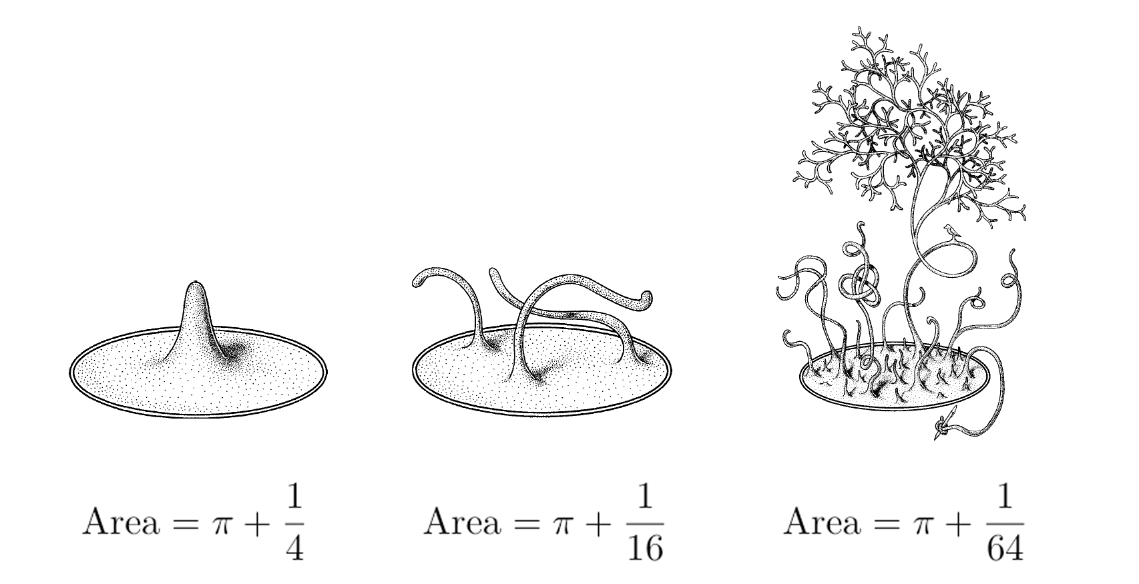
\includegraphics[scale=0.7]{images/area_minimizing.png}
        \caption{面积最小列, 但是没有收敛子列. 图片取自\cite{Morgan}}
        \label{figure_area_minimizing}
    \end{figure}
    \item 第二个问题是面积泛函是与参数选取无关的, 这意味着选取$\{u_k\}$后, 对于任意的微分同胚$\phi_k: \D \to \D$, $\Area(u_k\circ \phi_k(\D))= \Area(u_k(\D))$. 这种情况下, 我们也很难得到收敛子列.
\end{enumerate}
为了解决上面的问题, 我们将使用能量泛函而不是面积泛函. 当然, 首先我们需要说明的是, 对能量泛函求最小值和对面积泛函求最小值这两个问题是等价的(虽然对于能量泛函, 上述两个问题仍然存在, 但是我们较好的解决该问题的方法).
\begin{theorem}[Rado-Douglas] \label{rado_douglas}
    设$\gamma \subset \R^3$是可求长的Jordan曲线. 则存在映射$u \in \FG$使得 $\forall v \in \FG$, 
    \begin{equation}
        \Area(u(\D))\le \Area(v(\D)).
    \end{equation}
\end{theorem}
对于任意$u \in \FG$, 其面积与能量分别定义为
\begin{align}
    &\Area(u)=\int_\D\abs{u_x\wedge u_y} \\
    &\E(u)=\frac{1}{2}\int_\D\abs{u_x}^2+\abs{u_y}^2
\end{align}
简单计算可知
\begin{equation}\label{AleE}
    \Area(u)=\int_\D \sqrt{\abs{u_x}^2\abs{u_y}^2-\inner{u_x}{u_y}^2} \le \frac{1}{2}\int_\D \abs{u_x}^2+\abs{u_y}^2 \le\E(u).
\end{equation}
并且等号成立, 当且仅当$\abs{u_x}=\abs{u_y}, \inner{u_x}{u_y}=0$.
\par 记
\begin{align}
    &\AG=\inf\{\Area(v)\mid v \in \FG\}.\\
    &\EG=\inf \{\E(v)\mid v \in \FG\}.
\end{align}
\begin{definition}
    如果$u \in W^{1,2}(\mathbb{D},\R^3)$几乎处处满足$\inner{u_x}{u_y}=0$并且$\abs{u_x} = \abs{u_y}$, 则称$u$是几乎共形的.
\end{definition}
\begin{lemma}\label{ageg}
    $\AG=\EG$, 并且如果$u \in \FG$取到$\EG$, 则$u$是几乎共形的.
\end{lemma}
\begin{proof}
    由不等式\eqref{AleE}可知, $\AG \le \EG$.
    \par 对于反方向的, 设$u\in \FG$ 且$\Area(u) \le \AG + \epsilon$. 首先设$u$是浸入, 即$du$处处非退化. 设$(\D,g)$为$u$作用下的拉回度量, 即$g=du^*dx^2$, 由等温坐标的存在性可知, 存在光滑同胚$\phi: \D \to \D$使得$\phi$是$\mathbb{D} \to (\D,g)$ 之间的共形映射, 即$d\phi ^* g=\lambda^2dx^2$. 而$u\circ \phi$是共形浸入, 则有
    \begin{equation}
        \AG+\epsilon\ge \Area(u)=\Area(u\circ \phi)=\E(u\circ \phi) \ge \EG
    \end{equation}
    如果$du$有奇点, 那么我们定义$u^s: \D \to \R^5$, $u^s(x,y)=(u,sx,sy)\in \R^5$. 则$du^s$是非退化的. 像上面一样, 通过$u^s$拉回的度量为$du^*g_{\R^3}+s^2(dx^2+dy^2)$. 显然地, 
    \begin{equation}
        \Area(u^s)=\int_\D \det (du^*g_{\R^3}+s^2I)  \to \Area(u).
    \end{equation}
    \begin{equation}
        \E(u^s\circ\phi)=\int_\D \abs{(u^s\circ \phi)_x}^2+ \abs{(u^s\circ \phi)_y}^2 =\E(u\circ \phi)+s^2\E(\phi).
    \end{equation}
    因此, 当$s$足够小时, 我们有
    \begin{equation}
        \begin{split}
            \AG+2\epsilon \ge \Area(u)+\epsilon & \ge \Area(u^s\circ \phi)  \\
            &= \E(u^s\circ \phi)  \to \E(u\circ \phi) \\
            &\ge \EG.
        \end{split}
    \end{equation}
    若$E(u)=\EG$, 则$E(u)= \EG = \AG \le \Area(u)$, 则$E(u)=\Area(u)$. 由不等式\eqref{AleE}可知, $u$是几乎共形的.
\end{proof}
\begin{lemma}[Courant-Lebesgue引理] \label{courant_lebesgue}
    设$f \in W^{1,2}(\D,\R^3)$, $E(f) \le K$. 设$0 < \delta < 1$, $p \in \mathbb{D}$. 则存在$\rho \in (\delta, \sqrt{\delta})$ 使得$f\mid_{\P B(p,\rho) \cap \D}$是绝对连续的, 且$\forall z_1,z_2 \in \P B(p,\rho) \cap \D$, 成立 
    \begin{equation}
        \int_{\P B \cap \D} f_\theta^2 d\theta \le \frac{4K}{\log \rec{\delta}}
    \end{equation}
    以及
    \begin{equation}
        \abs{f(z_1)- f(z_2)} \le (8K\pi)^{\frac{1}{2}}(\log \frac{1}{\delta})^{-\frac{1}{2}}.
    \end{equation}
\end{lemma}
\begin{proof}
    在$p$点处引入极坐标$(r,\theta)$. 由于$f \in W^{1,2}$, 则几乎对于所有的$r$, $f$关于$\theta$是绝对连续的.  则Cauchy不等式, 
    \begin{equation}
        \begin{split}
            \abs{f(z_1)-f(z_2)} &\le \int_{\P B \cap \D} \abs{f_\theta(re^{i\theta})}d\theta \\
            & \le \sqrt{2\pi} (\int_{\P B\cap \D} f^2_\theta d\theta)^{\frac{1}{2}}.
        \end{split}
    \end{equation}
    而由于在极坐标下, $Df=f_r \P_r + \frac{1}{r^2}f_\theta \P_\theta$, 则
    \begin{equation}
        \int_{B \cap \D} (f_r^2 + \frac{1}{r^2}f_\theta^2)r drd\theta \le 2K.
    \end{equation}
    取$\rho$使得$\int_{\P B \cap \D} f^2_\theta(\rho e^{i\theta})$取到(几乎)最小, 则有
    \begin{equation}
        \int^{\sqrt{\delta}}_\delta \int_{\P B \cap \D}\frac{1}{r^2}f^2_\theta(\rho e^{i\theta}) rd\theta dr \le 2K.
    \end{equation}
    因此, 
    \begin{equation}
        \abs{f(z_1)-f(z_2)} \le \sqrt{2\pi} \frac{2K}{ \int^{\sqrt{\delta}}_\delta \frac{1}{r}} = \sqrt{8K\pi}(\log \frac{1}{\delta})^{-\frac{1}{2}}.
    \end{equation}
\end{proof}
\begin{remark}
    Courant-Lebesgue引理实际上只靠近边界的地方起作用, 将单位圆盘换成任意有限拓扑型的黎曼面$\Sigma$, 结论都是成立的(只需要取$\delta \le C=C(\Sigma)$). 后面在解决一般拓扑型的Plateau问题时, 我们还会多次用到Courant-Lebesgue引理.
\end{remark}
\begin{lemma}\label{three_point}
    设$p_1,p_2,p_3  \in \partial \D$是三个不同的点. 则对于任意三个点$\forall p'_1, p'_2, p'_3$, 存在唯一的共形同胚$\alpha: \D \to \D$使得$\alpha(p_i)=p'_i$. (假设$p_i, p'_i$在$\P \D$上都按逆时针排列)
\end{lemma}
\begin{proof}
    见任意复分析教材.
\end{proof}
\begin{lemma}\label{cut_curves}
    设$\gamma \subset \R^3$是长度有限的Jordan曲线, 则$\forall \epsilon > 0$, 存在$\lambda>0$使得$\forall p,q \in \gamma$, 如果$d(p,q)< \lambda$, 那么$\gamma-\{p,q\}$的两条曲线中, 只有一条的
    %直径(作为集合的直径)可以大于$\epsilon$. 
    长度可以大于$\epsilon$. 
\end{lemma}
\begin{proof}
    略.
\end{proof}
现在, 固定三个点$p_i \in \P D$, $q_i \in \gamma$. 设$K > 0$, 记
\begin{equation}
    \FG^K=\{u \in \FG\mid E(u) \le K, u(p_i)=q_i\}.
\end{equation}
\begin{lemma} \label{boundary_equicontinuous}
    $\FG^K\mid_{\P D}$是等度连续的.
\end{lemma}
\begin{figure}[ht]
    \centering
    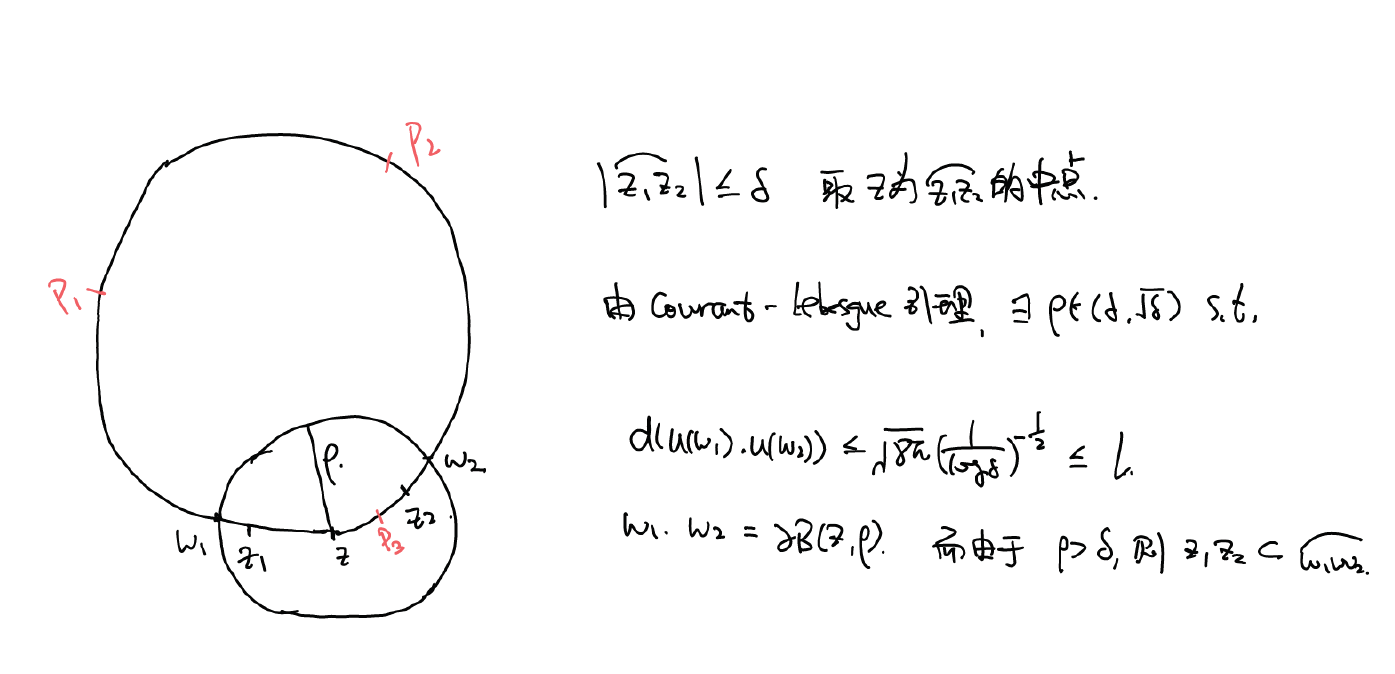
\includegraphics[scale=0.6]{images/courant_lebesgue.png}
    \caption{边界等度连续性}
    \label{equi_continuous}
\end{figure}
\begin{proof}
    我们选取$\epsilon$非常小, 使得$\gamma$中任意长度为$\epsilon$的曲线段都至多包含$\{q_i\}$中的一个点. 现在, 我们证明存在$\delta>0$, 使得如果$z_1,z_2 \in \P \D, \abs{z_1-z_2} \le \delta$, 则$\forall u \in \FG^K$, $\abs{u(z_1)-u(z_2)} \le \epsilon$.  
    \par 取$\delta$使得$(8K\pi)^{\rec{2}}(\log \rec{\delta})^{-\rec{2}} \le \lambda$, $\lambda$由引理\eqref{cut_curves}得到.  设$z_1,z_2 \in \P \D$.  设$\abs{z_1-z_2} \le \rec{\pi} \delta$, 用$\widehat{z_1z_2}$表示$\P \D - \{z_1,z_2\}$中较短的弧, 显然地, $\abs{\widehat{z_1z_2}} \le \delta$. 只要取$\delta$足够小, 就可以假设$\widehat{z_1z_2}$至多包含$\{p_i\}$中的一个点. 设$z$是弧$\widehat{z_1z_2}$的中点. 由引理\eqref{courant_lebesgue}, 存在$\rho \in (\delta, \sqrt{\delta})$使得$\forall u \in \FG^K$, 
    \begin{equation}
        d(u(w_1),u(w_2)) \le (8K\pi)^{\rec{2}}(\log \rec{\delta})^{-\rec{2}} \le \lambda.
    \end{equation}
    记$\{w_1,w_2\} = \P B(z,\rho) \cap \P \D$, 那么$u(w_1), u(w_2)$将$\gamma$分成两段, 其中较短的一段至多包含$\{q_i\}$中的一个点. 那么, 这一段的原像必定是$\widehat{w_1w_2}$.  而由于$\rho > \delta$, 则$z_1,z_2 \in \widehat{w_1w_2}$. 则$d(u(z_1),u(z_2)) \le \epsilon$.
\end{proof}
\begin{proof}[定理\eqref{rado_douglas}的证明]
    取$u_k \in \FG$ 且$E(u_k) \to \EG$. 由引理\eqref{three_point}, 存在$\phi_k$使得$u_k\circ \phi_k \in \FG^K$. 仍将$u_k\circ \phi_k$记为$u_k$.  用与$u_k$具有相同边界的调和函数替换$u_k$, 仍然记为$u_k$, 由于调和函数是能量最小的, 我们仍然有$E(u_k) \to \EG$.  由于$u_k$是调和的, 则
    \begin{equation}
        \max_{\D}\abs{u_k - u_l} = \max_{\P \D} \abs{u_k-u_l}.
    \end{equation}
    而根据引理\eqref{boundary_equicontinuous}, $u_k\mid_{\P \D}$ 包含一致收敛子列, 则$u_k$包含一致收敛子列. 设$u_k \to u$.  再选取$u_k$的子列, 使得$u_k \overset{\text{弱}W^{1,2}}{\longrightarrow} u$且$u_k \overset{L^2}{\longrightarrow} u$. 则由能量的下半连续性, 
    \begin{equation}
        E(u) \le \liminf E(u_k) \to \EG.
    \end{equation}
    最后, 由引理\eqref{ageg}, $\Area(u)=E(u)=\AG$.
\end{proof}
\ifcomment
    \begin{remark}
        如果没有三点正规化的话, 不影响等度连续性, 但是得到的极限可能是常值函数.
    \end{remark}
\fi
\section{The Annulus Case}
现在, 我们考虑复杂一点的情况. 设$\Gamma=\gamma_1 \cup \gamma_2$是两条简单闭曲线的并. 是否存在以$\Gamma$为边界的极小曲面?  
\par 与圆盘的情况不同的是,  并不总是能找到以$\Gamma$为边界的极小曲面.  这里我们给出一个反例.  设$\Sigma$为Catenoid, 即$\Sigma=\{\cosh^2 z = x^2+y^2\}$.  设$\Sigma_a= a\Sigma$.  那么, 当$a \to +\infty$时,  $\Sigma_a \to \emptyset$.  $a\to 0$时, $\Sigma_a \to 2\{z=0, x^2+y^2\ne 0\}$.  简单计算易知,  存在锥体$C_\lambda=\{x^2+y^2< \lambda^2z^2\}$使得$C_\lambda\cap \Sigma=\emptyset$.  而由于$C_\lambda$在相似变换下是不变的, 则$\forall \Sigma_a \cap C_\lambda = \emptyset$.  分别记$C^+_\lambda=C_\lambda \cap \{z>0\}$, $C^-_\lambda=C_\lambda \cap \{z<0\}$. 
\begin{figure}[ht]
    \centering
    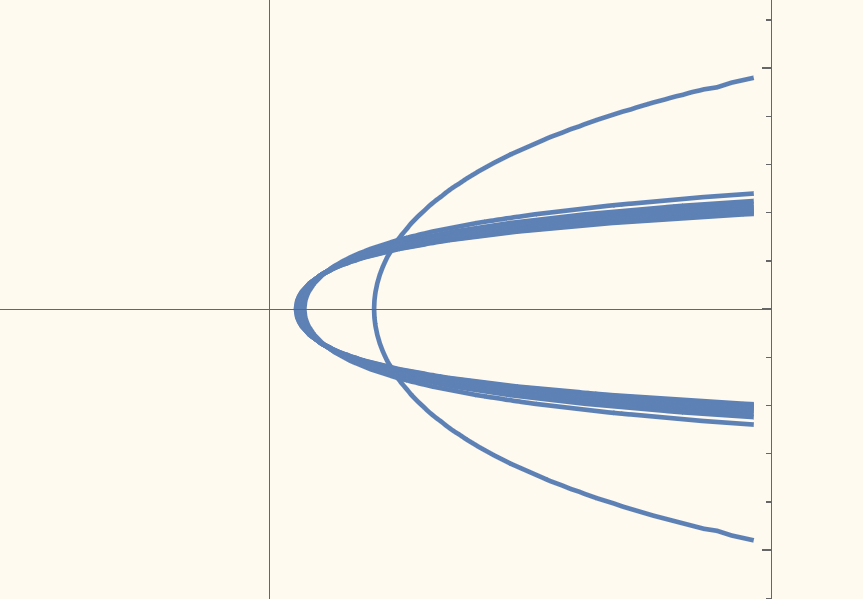
\includegraphics[scale=0.4]{images/sequence_of_catenoid.png}
    \caption{$\Sigma_a$与$C_\lambda$没有交集.}
    \label{label}
\end{figure}
%\lstinputlisting[language=Mathematica]{mathematica/sequence_of_catenoid.m}
\begin{definition}
    设$\Sigma$是二维流形. 称$\Sigma$是双连通的, 如果$\Sigma$同胚于$\{1< \abs{z}< 2\}$.  双连通曲面有时我们也会称为annulus型曲面.
\end{definition}
\begin{proposition}
    设$\Gamma=\gamma_1 \cup \gamma_2$, $\gamma_1 \subset C^+_\lambda, \gamma_2 \subset C^-_\lambda$. 则不存在以$\Gamma$为边界的双连通极小曲面.
\end{proposition}
\begin{proof}
    设这样的极小曲面存在, 记为$M$.  显然地, $a \to 0$时,  $\Sigma_a \cap M \ne \emptyset$.  $a \to \infty$时, $\Sigma_a \cap M = \emptyset$. 那么存在$a$使得$\Sigma_a$恰好与$M$相切且位于$M$的同一侧, 这将与最大值原理矛盾.
\end{proof}

在此, 我们指出, 在解决给定拓扑型的Plateau问题时, 我们所会碰到的核心困难在于拓扑型的退化. 如图\eqref{figure_annulus_minimizing}我们要寻找由两个圆盘围出的同胚于环面的极小曲面(图一图二均为两个环面, 且面积变小. 图三为两个圆盘). 当我们取面积递减的曲面序列的时候, 虽然所取的每一个曲面都同胚于环面, 但是最终得到的极限却是两个圆盘. 这种现象便是拓扑型的退化.即, 取极限后无法保证得到的曲面的拓扑是我们想要的.
\begin{figure}[ht]
    \centering
    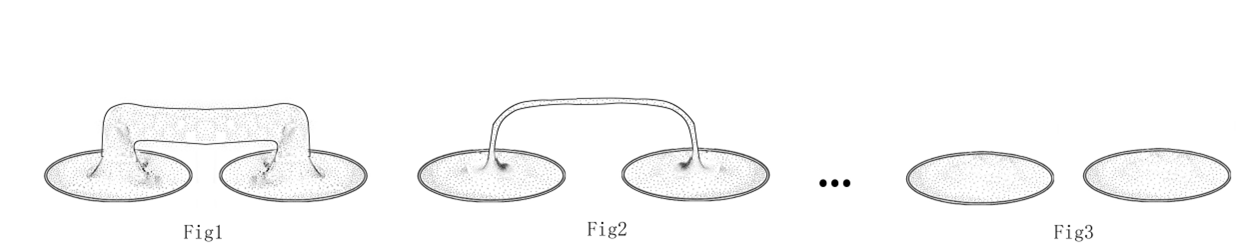
\includegraphics[scale=0.8]{images/annulus_minimizing.png}
    \caption{拓扑型的退化}
    \label{figure_annulus_minimizing}
\end{figure}

\par 解决annulus型的Plateau问题, 与disk型的另一个区别在于, 在选取参数域的时候, 由于所有的单连通区域(除了$\mathbb{C}$及$\S^2$)都是共形等价的, 我们可以假设参数域就是单位圆盘$\D$. 然而在双连通的情况, 由定理\eqref{uniformization_annulus}, 双连通域之间并不共形等价, 这样我们在选取参数域的时候就多了一个参数(区域的共形模, 参考定义\eqref{conformal_modulus}).  
\begin{remark}
    $B_{1,e^s}=\{1<\abs{z}< e^s\}$与$\S^1\times (0, s)\subset \R^3$是共形等价的,  我们将选取$\S^1\times (0,s)$形的区域作为参数域.
\end{remark}

\begin{lemma} \label{boundary_energy}
    设$\phi: \S^1 \to \R$是绝对连续的,  设$u\in C(\D)$是调和函数并且$u\mid_{\P \D}=\phi$. 则
    \begin{equation}
        \int_{\P \D} \abs{\nabla u}^2dxdy \le \int_{\S^1} \abs{\phi_\theta}^2d\theta.
    \end{equation}
\end{lemma}
\begin{proof}
    设$(r,\theta)$是极坐标. 设$c_n=\rec{2\pi}\int_{\S^1} \phi(\theta)e^{-i n \theta}d\theta$. 则$u, u_r$具有展开式
    \begin{align}
        &u(r,\theta)=\sum_{-\infty}^{+\infty}c_n r^{\abs{n}}e^{in\theta}, \label{fourier_u} \\
        &u_r(r,\theta)=\sum_{-\infty}^{+\infty}c_n\abs{n} r^{\abs{n}-1}e^{in\theta}. \label{fourier_ur}\\
    \end{align}
    由散度定理, 并将\eqref{fourier_u},\eqref{fourier_ur}代入计算可知
    \begin{equation}
        \begin{split}
            \int_{{\abs{z}\le r}}\abs{\nabla u}^2dxdy & =\int_{\{\abs{z}=r\}}uu_rd\theta\\
            &=2\pi \sum_{-\infty}^{+\infty}\abs{n}r^{2n}\abs{c_n}^2.
        \end{split}
    \end{equation}
    另外, 有
    \begin{equation}
        \int_{\S^1} \abs{u_\theta}^2 = 2\pi\sum_{-\infty}^{+\infty} \abs{n}^2\abs{c_n}^2.
    \end{equation}
    令$r \to 1$即可.
\end{proof}
\begin{lemma} \label{fill_hole}
    设 $\delta <1$. 定义
    \begin{equation}
        \eta_\delta(r)=\left\{
            \begin{aligned}
                &1 \s r \ge \sqrt{\delta}, \\
                &1+\frac{\log \sqrt{\delta}- \log r}{ \log \sqrt{\delta}} \s \delta \le r \le \sqrt{\delta}\\
                &0 \s r \le \delta
            \end{aligned}
            \right.
    \end{equation}
    设$u \in W^{1,2}(\Sigma) \cap C(\Sigma)$. 定义
    \begin{equation}
        u_\delta(z)=\left\{
            \begin{aligned}
                & u(z) \s \abs{u(z)-p} \ge \sqrt{\delta} \\
                & p+ \eta_\delta(\abs{u(z)-p})(u(z)-p)
            \end{aligned}
        \right.
    \end{equation}
    则当$\delta \to $时, $E(u_\delta) \to E(u)$.
\end{lemma}
\begin{figure}[h]
    \centering
    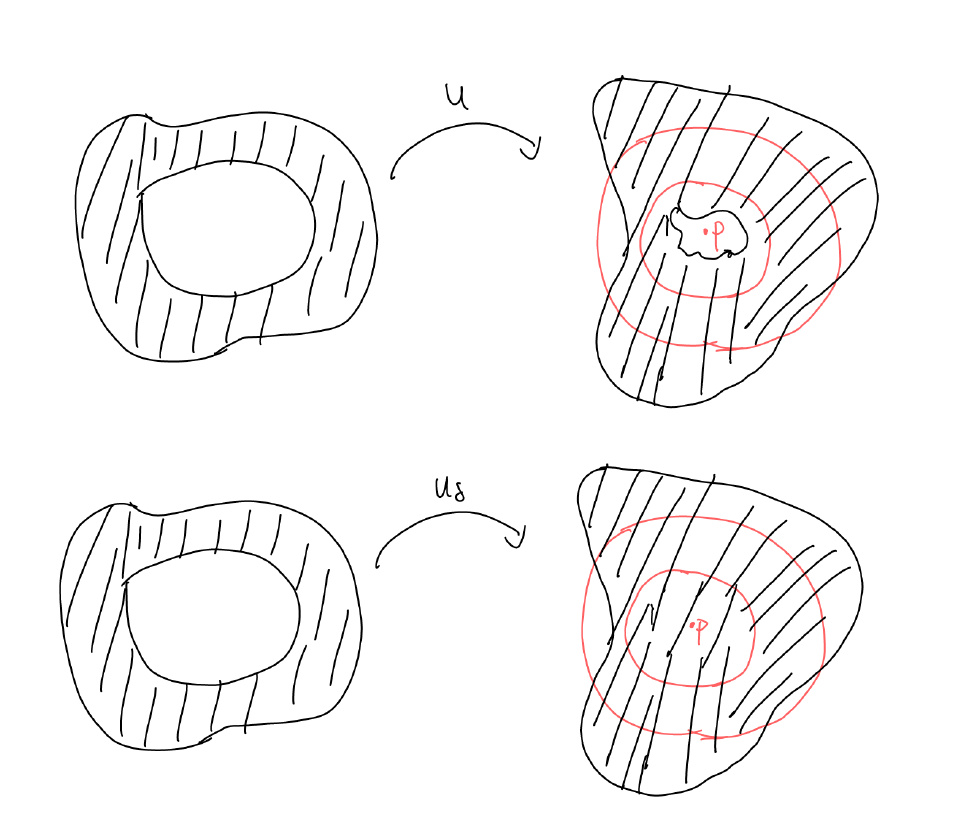
\includegraphics[scale=0.5]{images/contraction.png}
    \caption{$u_\delta$填补了$u$的像中的``空洞"}
    \label{aaaanonlabel}
\end{figure}

\begin{proof}
    设$\Omega_\delta=\{\abs{u(z)-p} < \sqrt{\delta}\}$. 则 $E(u_\delta)=E(u,\Sigma-\Omega_\delta)+E(u_\delta, \Omega_\delta)$. 我们计算第二项.
    \begin{equation}
        \begin{split}
            E(u_\delta, \Omega_\delta) & =\rec{2}\int_{\Omega_\delta} {\eta'}^2(\abs{u(z)-p})\abs{Du}^2+\eta^2(\abs{u(z)-p}) \abs{Du}^2 dv_g\\
            &\le \rec{2}\int_{\Omega_\delta} \frac{\abs{Du}^2}{(\log\sqrt{\delta}\delta)^2} +\abs{Du}^2dv_g
        \end{split}
    \end{equation}
    因此, 
    \begin{equation}
        \abs{E(u)-E(u_\delta)} \le \frac{1}{\delta\log\sqrt{\delta}}\int_{\Omega_\delta} \abs{Du}^2dv_g \to 0.
    \end{equation}
\end{proof}
对于annulus型的Plateau问题, Douglas的结果可以陈述为:
\begin{theorem}
    设$\Gamma= \gamma_1 \cup \gamma_2 \subset \R^3$是两条不相交的简单闭曲线的并. 设存在以$\Gamma$为边界的双连通曲面$M$使得
    \begin{equation} \label{douglas_condition_annulus}
        \Area(M) < \AA_{\gamma_1}+\AA_{\gamma_2}.
    \end{equation}
    则存在以$\Gamma$为边界的双连通的极小曲面.
\end{theorem}
\begin{proof}
    设$u_k: \Sigma \to \R^3$, $E(u_k) \to \EE_{\Gamma}$.  记$K=\EE_{\Gamma}+1 < +\infty$. 这里, $\Sigma_k = \S\times (0,s_n)$. 现在,我们证明: 存在子列使得 $s_n \to s >0$.  $\Sigma_n$上的参数记为$(\theta,r)$. $\theta \in \S^1, r \in (0,s_k)$.
    \begin{claim}
        $\{s_k\}$有严格正的下界.
        \begin{subproof}
            记$d=d(\gamma_1,\gamma_2)>0$. $\forall \theta$, 设$\alpha$ 为直线$\theta \times (0, s_k)$. 显然地, $l_{u_k(\alpha)} \ge d$. 则由Cauchy不等式
            \begin{equation}
                d^2 \le (\int^{s_k}_0 \abs{du_k \alpha'} ds)^2 \le s_k \int^{s_k}_0 (\PTT{u_k})^2dr.
            \end{equation}
            于是, 有
            \begin{equation}
                \frac{2\pi d^2}{s_k} \le \int_{\S^1}\int^{s_k}_0 (\PTT{u_k})^2 drd\theta \le E(h) \le K.
            \end{equation}
            则$s_k \ge \frac{2\pi d^2}{K}$.
        \end{subproof}
    \end{claim}
    \begin{claim}
        $\{s_k\}$有上界(不等于$+\infty$).
        \begin{subproof}
            反证法.  设$s_k \to +\infty$. 由于$\E(u_k) \le K$,  则存在$\rho_k \in (0, s_k)$使得
            \begin{equation}
                s_k\int_{\S^1 \times \{\rho_k\}} (\PTT{u_k})^2(\theta,\rho_k) d\theta \le K.
            \end{equation}
            \begin{figure}[!h]
                \centering
                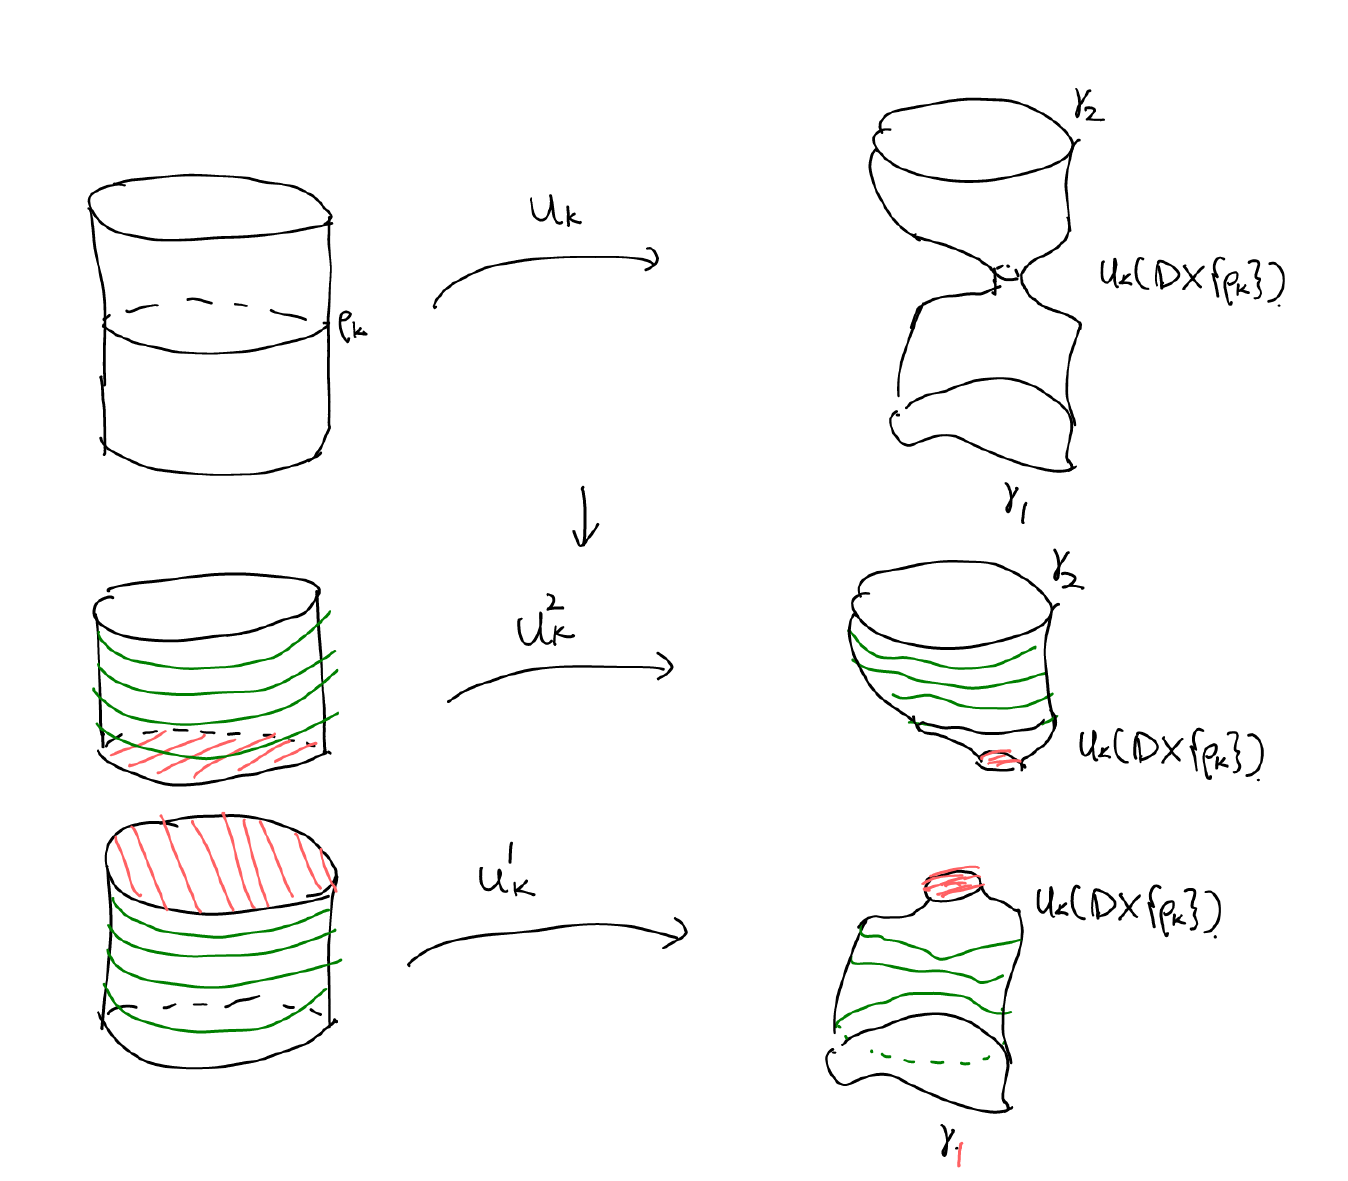
\includegraphics[scale=0.6]{images/closed_degenerate.png}
                \caption{曲线的退化}
                \label{closed_degenerate}
            \end{figure}
            则有$\int_{\S^1\times \{\rho_k\}} (\PTT{u_k})^2(\theta,\rho_k) d\theta  \to 0$. 实际上这意味着拓扑型的退化. 设$\gamma$为曲线$\S^1 \times \{\rho_k\}$并取其弧长参数, 则
            \begin{equation}
                l_\gamma = \int_\gamma\abs{\gamma'}ds \le (2\pi\int_\gamma \abs{\gamma'}^2ds^2) \to 0.
            \end{equation}
            这意味着出现了图\eqref{figure_annulus_minimizing}中的情况.  现在我们利用Douglas条件\eqref{douglas_condition_annulus}来说明这是不可能发生的.
            记$\D_{\rho_k}=\D \times \{\rho_k\}$. 现在以$u_k(\rho_k,\theta)$为边界值, 由引理\eqref{boundary_energy}可知, 存在函数$f_k: \D_{\rho_k} \to \R^3$使得$E(f_k) \to 0$.  定义
            \begin{equation}
                \Sigma^1_k= \S^1 \times (0,\rho_k) \cup \D_{\rho_k},\s \Sigma^2_k=\S^1\times (\rho_k,s_k) \cup \D_{\rho_k}.
            \end{equation}
            显然地, $\Sigma^1_k, \Sigma^2_k$都是单连通的. 现在我们定义两个新的映射:
            \begin{equation}
                {u}_k^1: \Sigma^1_k \to \R^3.  \s  {u}_k^1=\left\{
                    \begin{aligned}
                        &u_k\s x \in \S^1 \times (0,\rho_k),\\
                        &f_k\s x \in \D_{\rho_k}.
                    \end{aligned}
                \right.
            \end{equation}
            \begin{equation}
                {u}_k^2: \Sigma^2_k \to \R^3.  \s  {u}_k^2=\left\{
                    \begin{aligned}
                        &u_k\s x \in \S^1 \times (\rho_k, s_k),\\
                        &f_k\s x \in \D_{\rho_k}.
                    \end{aligned}
                \right.
            \end{equation}
            则$E({u}_k^1)+E({u}_k^2) \le E(u_k)+2E(f_k)$. 而显然地, ${u}_k^1(\P \Sigma^1_k) = \gamma_1$,${{u}}_k^2(\P \Sigma^2_k)= \gamma_2$. 则
            \begin{equation}
                \begin{split}
                    \AA_{\gamma_1}+\AA_{\gamma_2} = \EE_{\gamma_1}+\EE_{\gamma_2} & \le  \lim E({u}_k^1)+E({u}_k^2)  \\
                    &\le \lim E(u_k) + 2E(f_k) \to \EE_\Gamma=\AA_\Gamma.
                \end{split}
            \end{equation}
            这与条件\eqref{douglas_condition_annulus}矛盾.
        \end{subproof}
    \end{claim}
    设$\Sigma_k \to \Sigma = \S^1 \times (0,s)$. 同时, 通过变换$(x,r) \to (x,\frac{s_k}{s}r)$, 我们可以假设$u_k$定义在$\Sigma$上.
    \begin{claim}
        $u_k\mid_{\P \Sigma}$是等度连续的.
        \begin{subproof}
            我们只考虑$u_k\mid_{\P \D}$的等度连续性即可.  设$\epsilon_k \to 0$, 由引理\eqref{courant_lebesgue}, $\forall p \in \P \D, \delta>0$, 存在$\rho_k \in (\delta,\sqrt{\delta})$使得
            \begin{equation}
                l_{u_k(\P B(p,\rho_k) \cap \Sigma)} \le \sqrt{8K\pi}(\log(\rec{\delta}))^{-\rec{2}}.
            \end{equation}
            记$\beta_k=\P B(p,\rho_k) \cap \D$. $\beta$的端点将$\P \D$分成两部分, 其中短的一部分记为$C_k'$, 长的部分记为$C_k''$. $u_k(\beta_k)$的两个端点将$\gamma_1$分成两部分, 其中短的记为$\gamma_{1k}'$, 长的记为$\gamma_{1k}''$(``长'', ``短''是在引理\eqref{cut_curves}意义下的). 如同引理\eqref{boundary_equicontinuous}的证明中一样, 由Courant-Lebesgue引理,  如果能说明$\forall k$, $u_k(C_k')=\gamma_{1k}'$, 那么$u_k$是等度连续的.  反证法. 设$u_k(C_k')=\gamma_{1k}'', u_k(C_k'')=\gamma_{1k}'$. 由引理\eqref{cut_curves}, $l_{u(\beta_k)\cup \gamma_{1k}'} \le \epsilon_k \to 0$.  注意到, $u_k(\beta_k) \cup \gamma_{1k}'$实际上是$u_k(\Sigma)$的core curve(也就是$u_k(\Sigma)$基本群的生成元), 这意味着出现了图\eqref{figure_annulus_minimizing}中的情况. 现在我们将构造两个映射$u_{1k}, u_{2k}$, 这两个映射都定义在单连通区域上, 且分别将两个单连通区域的边界映为$\gamma_1, \gamma_2$. 
            \begin{figure}[ht]
                \centering
                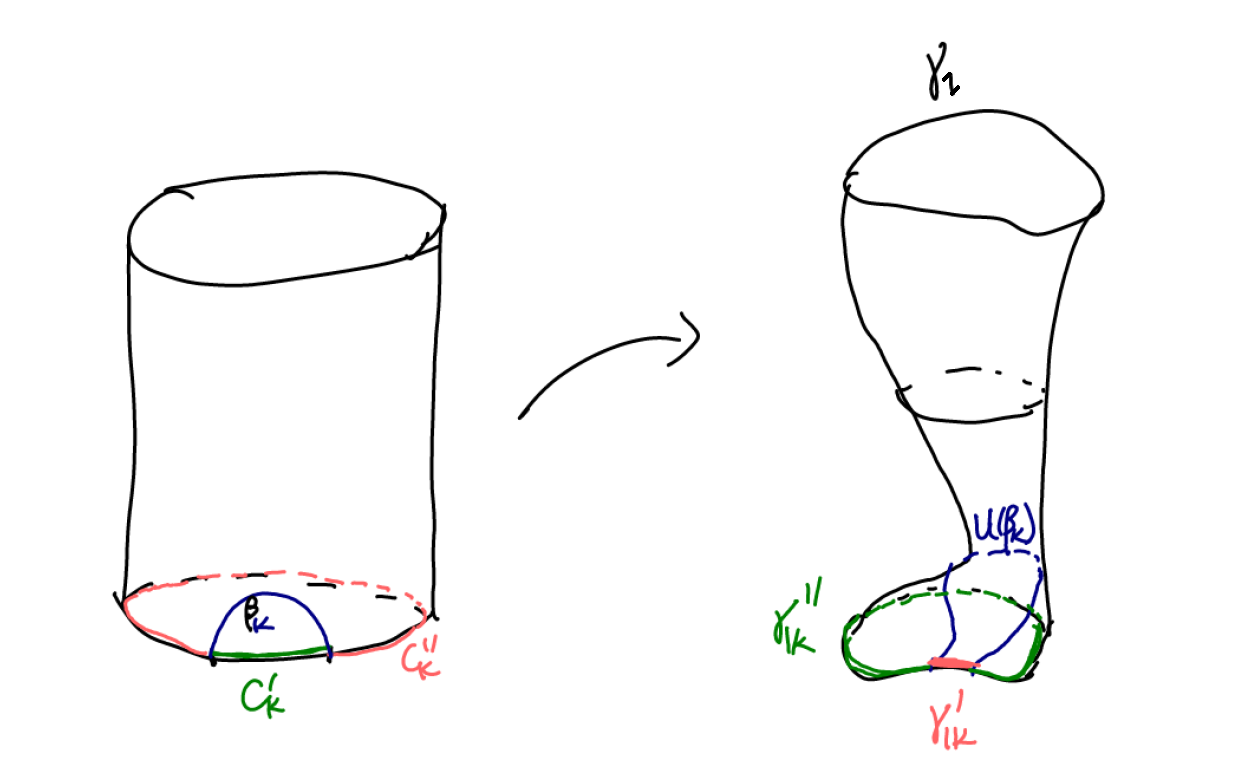
\includegraphics[scale=0.4]{images/pinch.png}
                \caption{设在$u_k$映射下, ``短''的弧被映射为``长''的弧}
                \label{pinch}
            \end{figure}
            \par 首先, 我们将曲面$\Sigma$沿着$\beta_k$剪开, 其中包含边界$\S^1\times \{s\}$的部分记为$\Sigma_k''$, 由$\beta_k$及$C_k'$围出的区域记为$\Sigma_k'$. 在$\Sigma_k''$的边界$C_k''\cup \beta$上, 粘贴上一个圆盘, 这样就得到了一个单连通区域, 记为$\tilde{\Sigma}_k''$.  %现在我们分别在$\Sigma_k'$及$\tilde{\Sigma}_k''$上定义两个映射.
            \par 取$q \in \R^3$使得$d(q, u_k(\beta_k) \cup \gamma_{1k}') < 2\epsilon_k$.  将引理\eqref{fill_hole}应用到$u_k, 2\epsilon_k, q$上(取$u=u_k, p=q, \delta=\epsilon_k$), 得到新的映射记为$u_{2k}$. 注意到$u_{2k}$将$\beta_k \cup C_k''$的邻域映射到点$q$. 在$\tilde{\Sigma}''_k-\Sigma''_k$上将$u_{2k}$定义常值$q$, 那么就得到了$u_{2k}: \tilde{\Sigma}_k'' \to \R^3, u_{2k}({\P \tilde{\Sigma}_k''})=\gamma_2$.
            \begin{figure}[ht]
                \centering
                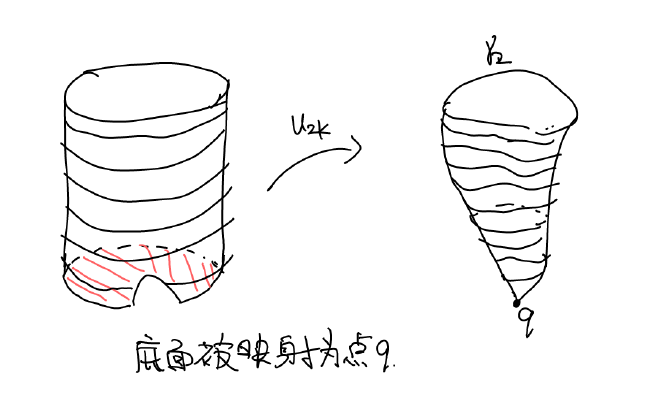
\includegraphics[scale=0.7]{images/u2k.png}
                \caption{$u_{2k}$}
                \label{u2k}
            \end{figure}
            \par  现在我们定义$u_{1k}$. 由于$\Sigma_k'$是单连通的, 我们将$\Sigma_k'$共形映射为下半单位圆盘, 并将$\beta_k$映射为$\{\abs{z}=1\} \cap \D$.  设$\gamma_{1k}'$的长度为$l_k$, 取$\gamma_{1k}'$的弧长参数化, 现在我们定义$\phi_k: \P \D \cap \{\Im(z)>0\} \to \R^3$, 对于$z \in \S^1 \cap \{\Im(z) >0\}$, 记$\theta(z)=\text{Arg}(z)$.
            \begin{equation}
                \phi_k=\left\{
                    \begin{aligned}
                        & u_k(z) \s z \in \{\Im(z)=0\}, \\
                        & \gamma_{1k}'(\frac{l_k}{\pi}\theta(z)) \s z \in \S^1 \cap \{\Im(z)>0\}.
                    \end{aligned}
                \right.
            \end{equation}
            \begin{figure}[!h]
                \centering
                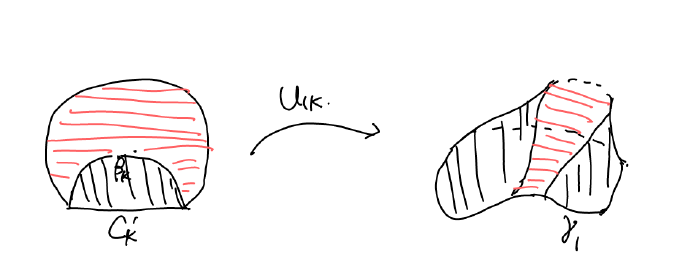
\includegraphics[scale=0.8]{images/u1k.png}
                \caption{$u_{1k}$}
                \label{u1k}
            \end{figure}
            由Courant-Lebesgue引理及$l_k\to 0$可知, $\int_{\S^1} \abs{\phi_k'(\theta)}^2 d\theta \to 0$.  设$v_k$是以$\phi_k$为边界值的调和函数. 则由引理\eqref{boundary_energy}, $E(v_k) \to 0$. 定义$u_{1k}$如下
            \begin{equation}
                u_{1k}(z)=\left\{
                    \begin{aligned}
                        &u_k(z)\s \Im(z)>0, \\
                        &v_k(z)\s \Im(z) <0.
                    \end{aligned}
                \right.
            \end{equation}
            则$u_{1k}(\S^1)= \gamma_1$. 注意到, $u_{1k}, u_{2k}$的定义域都是单连通的. 而根据我们的构造, 有
            \begin{equation}
                \EE_{\gamma_1}+\EE_{\gamma_2}\le \lim E(u_{1k})+E(u_{2k})= \lim E(u_k)= \EE_{\Gamma}.
            \end{equation}
            这等价于$\AA_{\gamma_1}+\AA_{\gamma_2} \le \AA_\Gamma$, 与Douglas条件\eqref{douglas_condition_annulus}矛盾.
        \end{subproof}
    \end{claim}
    现在有了边界上的等度连续性, 剩下的只需重复定理\eqref{rado_douglas}的证明即可.
\end{proof}
\section{The General Case}
\subsection{双曲几何}
我们只关心二维的双曲几何.
\subsubsection{定义及基本性质}
\begin{definition}
    称曲率为$-1$的度量称为双曲度量. 
\end{definition}
我们提到双曲空间时, 一般指赋予完备双曲度量的单连通空间.  双曲空间的常用模型是单位圆模型和上半平面模型.
\begin{enumerate}
    \item 单位圆盘模型: 单位圆盘$\D$赋予度量$\frac{2}{1-\abs{z}^2}\abs{dz}$.
    \item 上半空间模型: 上半平面$\HH=\{y>0\}$赋予度量 $\frac{1}{y}\abs{dz}$.
\end{enumerate}
\par 从现在开始, 在本节中, 当我们提到$\D$及 $\HH$时, 总是赋予其双曲度量. 
\begin{proposition}
    $\D$与$\HH$都是完备的黎曼流形.
\end{proposition}
\begin{lemma}\label{d2h}
    $u(z)=\frac{i(1+z)}{1-z}$是$\D \to \HH$之间的等距同构.
\end{lemma}
\begin{proof}
    直接计算.
\end{proof}
在复分析中, 我们知道单位圆盘的共形同构群是$\aut(\D)$.
\begin{equation}
    \aut(\D)=\{e^{i\theta}\frac{z_0-z}{1-\bar{z_0}z} \mid \theta \in \mathbb{S}^1, z_0 \in \D\} .
\end{equation}
而对于上半空间, 设$\text{SL}(2,\R)=\{\begin{pmatrix}
    &a\s b \\
    &c\s d
\end{pmatrix}\}\mid a,b,c,d \in \R, ad-bc=1\}$. 
记
\begin{equation}
    \psl(2,\R)=\text{SL}(2,\R)/\{\pm 1\}.
\end{equation}
那么上半空间的共形同构群为$\psl(2,\R)$. 对于$\gamma\in \psl(2,\R)$, $\gamma=\begin{pmatrix}
    &a\s b\\
    &c\s d
\end{pmatrix}$, $\gamma$在$\HH$上的作用方式为:$\gamma(z)=\frac{az+b}{cz+d}$.
\begin{theorem}
    设$\D$及$\HH$赋予双曲度量, 则
    \begin{enumerate}
        \item $\aut(\D)$是$\D$的等距同构群. 
        \item $\psl(2,\R)$是$\HH$的等距同构群.\label{auth2}
    \end{enumerate}
\end{theorem}
\begin{proof}
    由引理\eqref{d2h}, 我们只需要证明其中一个结论即可. 我们证明\eqref{auth2}. 
    \par 设$\gamma: \HH \to \HH$是等距同构, 那么显然$\gamma$是保持角度的, 即有$\gamma \in \psl(2,\R)$.
    \par 反之, 设$\gamma=\begin{pmatrix}
        &a \s b\\
        &c \s d
    \end{pmatrix}$.  直接计算可知
    \begin{equation}
        \begin{split}
            \rec{\Im(\gamma(z))}\abs{d\gamma(z)}&=\rec{\Im(\gamma(z))}\abs{\gamma'(z)}\abs{dz} \\
            &=\rec{\Im(\frac{(az+b)(c\bar{z}+d)}{\abs{cz+d}^2})} \abs{\frac{(cz+d)a-(az+b)c}{(cz+d)^2}} \abs{dz} \\
            &=\rec{\Im(z)\abs{dz}}
        \end{split}
    \end{equation}
    即$\gamma$是$\HH \to \HH$的等距.
\end{proof}
\begin{lemma}
    $\D$中任意两个点之间的测地线是唯一的.
\end{lemma}
\begin{proof}
    设$\alpha,\beta$是具有相同端点的测地线, 设它们围出的区域为$\Omega$, 在两个点端处的$\alpha$,$\beta$所成的外角度为$a,b \in $, 则由Gauss-Bonnet公式,
    \begin{equation}
        \int_\Omega -1dv_g+a+b=2\pi.
    \end{equation}
    则$\int_\Omega -1dv_g \ge 0$, 于是$\Omega =\emptyset$.
\end{proof}
\begin{theorem}
    $\D$中的完备测地线是通过原点的直线, 或者与$\D$垂直的圆弧.
\end{theorem}
\begin{proof}
    由度量$\frac{2}{1-\abs{z}^2}\abs{dz}$的对称性可知, 任意通过原点的直线是测地线. 设$l \subset \D$是完备测地线. 设$p\in l$. 记$\gamma\in \aut(\D), \gamma=\frac{p-z}{1-\bar{p}z}$, 则$\gamma$是将$p$点映射为原点的等距映射, 那么$\gamma(l)$是过原点的直线. 而任意的$\mobius$变换都将直线或圆周映射为直线或圆周, 因此$l$是直线或圆周. 由于$\gamma^{-1}$是保持角度的, 而$\gamma(l)$与$\S^1$垂直, 则$l$与$\gamma^{-1}(\S^1)$垂直. 又知$\gamma^{-1}(\S^1)=\S^1$, 则 $l$与$\S^1$垂直.
\end{proof}
\begin{theorem}
    $\HH$中的完备测地线是与实轴垂直的直线.
\end{theorem}
\begin{proof}
    由引理\eqref{d2h}易知.
\end{proof}
\begin{remark}
    双曲空间的两种模型, $\D$与$\HH$作为黎曼流形是完全相同的, 后面我们会根据需要选择合适的模型. 唯一需要指出的是, 在单位圆盘模型中,  双曲空间的边界就是单位圆周$\S^1$. 在上半空间模型中, 双曲空间的边界为$\R \cup \{\infty\}$.  需要注意, $\R\cup \{\infty\}$是同胚于$\S^1$的.  引理\eqref{d2h}中的$\mobius$变换恰好是将$\S^1$映射为$\R \cup \{\infty\}=\RR$.  在后文中, 我们用$\HC$表示$\HH \cup \RR$或者$\D \cup \S^1$.
\end{remark}
\begin{corollary} \label{unique_geodesic}
    对于任意两个点$p,q \in \HC$, 存在唯一的连接$p,q$的测地线.
\end{corollary}
\subsubsection{$\mobius$变换的分类}
\begin{proposition}
    设$\gamma \in \psl(2,\R)$, 如果$\gamma$有: 一个内部不动点及一个边界不动点, 或者有三个边界不动点, 则$\gamma$一定是恒同映射.  
\end{proposition}
\begin{proof}
    略.
\end{proof}
根据$\mobius$变换不动点的个数及位置, 可以将$\psl(2,\R)$中的元素分为三类. 
\begin{enumerate}
    \item $\gamma$有一个内部不动点, 则称$\gamma$为椭圆型.
    \item $\gamma$只有一个边界不动点, 则称$\gamma$为抛物型.
    \item $\gamma$有两个个边界不动点, 则称$\gamma$为双曲型.
\end{enumerate}
\begin{definition}
    称$\alpha, \beta \in \psl(2,\R)$共轭的, 如果存在$\gamma \in \psl(2,\R)$使得$\alpha=\gamma \circ \beta \circ \gamma^{-1}$.
\end{definition}
\par 由于在解决Plateau问题的过程中不会碰到椭圆及抛物型元素, 这里我们只对双曲型元素做详细的解释. 
\par 设$\gamma\in \psl(2,\R)$是双曲型元素, 设$p,q \in \RR$是其两个不动点.  根据推论\eqref{unique_geodesic},  存在唯一的连接$p,q$的测地线, 记为$\overline{pq}$. 由于$\gamma$是等距同构, 那么$\gamma(\overline{pq})$也是测地线, 因此必然有$\gamma(\overline{pq})=\overline{pq}$.  即, $\gamma$保持连接它的两个不动点之间的测地线不变. 这条测地线称为\textbf{双曲型元素$\gamma$的轴}. 取$\alpha\in \psl(2,\R)$将$p$映射为$0$点, 将$q$映射为$\infty$. 那么$\alpha\circ\gamma \circ \alpha^{-1}$ 将保持$0$与$\infty$不动. 
设$\beta= \alpha \circ \gamma \circ \alpha^{-1}=\begin{pmatrix}
    &a\s b\\
    &c\s d
\end{pmatrix}$.  将$\beta(0)=0, \beta(\infty)=\infty$代入可知, $b=c=0$.  记$\lambda=\frac{a}{d}$, 则$\beta(z)=\lambda z$.
于是我们得到:
\begin{proposition}
    设$\gamma \in \psl(2,\R)$是双曲型元素, 则存在$\lambda >0$使得$\gamma$共轭于$z \mapsto \lambda z$
\end{proposition}
%\begin{definition}
%    设$X$为拓扑空间, 设$G\times X\to X$是群$G$在集合$X$上的作用.  称$G$在$X$上的作用是纯不连续的, 如果$\forall x \in X$, 存在点$x$的邻域$U$使得$\forall g \in G$, $g(U) \cap U=\emptyset$.
%\end{definition}
%\begin{proposition}
%    设$G\times X \to X$的作用是纯不连续的, 则投影映射$X \to X/G$覆盖映射.
%\end{proposition}
%\begin{proof}
%    参考\cite{munkres}.
%\end{proof}
\begin{definition}
    设$\Gamma \subset \psl(2,\R)$是子群.  称$\Gamma$是Fuchsian群/(离散群), 如果$\forall z \in \HH$, 都存在$z$点的邻域$U$, 使得$\forall \gamma \in \Gamma$, $\gamma(U) \cap U=\emptyset$.
\end{definition}
\begin{definition}
    设$\Gamma \subset \psl(2,\R)$是Fuchsian群. $\forall z \in \HH$, 称集合$\{\gamma(z)\mid \gamma \in \Gamma\}$为点 $z$的轨道. 设$z_1, z_2\in \HH$. 称$z_1,z_2$等价,  如果$z_1,z_2$在同一个点的轨道中, 记为$z_1\sim z_2$. 容易验证, 这确实是一个等价关系.  记$\HH/\Gamma$所有轨道的集合, 即商空间$\HH/\sim $, 并赋予商拓扑.
\end{definition}
\begin{theorem}\label{covering}
    设$\Gamma$是Fuchsian群. 则投影映射$\pi: \HH \to \HH/\Gamma$是覆盖映射, 并且$\pi_1(\HH/\Gamma)=\Gamma$.
\end{theorem}
\begin{proof}
    这是一个纯拓扑的结果, 跟双曲几何本身没有关系. 参考\cite[定理81.5]{munkres}.
\end{proof}
\par 设$\Gamma$是Fucisian群, 由于$\pi \HH \to \HH/\Gamma$是覆盖映射, 我们可以通过局部坐标将$\HH$上的双曲度量下降到$\HH/\Gamma$上. 对于$p \in \HH/\Gamma$, 取其邻域$U$使得$U$同胚于$\pi^{-1}(U)$的每一个连通分支.  任取$\pi^{-1}(U)$的一个连通分支, 记为$V\subset \HH$. 将$\pi^{-1}: U \to V$看作$\HH/\Gamma$上的坐标卡, 将$V\subset \HH$中的度量拉回到$U$中. 这样便在$\HH/\Gamma$上定义了一个双曲度量. $\Gamma$中的每个元素都是$\HH$的等距变换保证了我们在$\HH/\Gamma$上定义的度量与坐标的选取没有关系.
\par 设$\gamma(z): z\mapsto \lambda z$, $\lambda>1$.  设$\Gamma=\left<\gamma\right >$是由$\gamma$生成的循环群.  我们来看一下曲面$\HH/\Gamma$的拓扑及几何.  我们记
\begin{equation}
    \Omega_\lambda=\{1< \abs{z}< \lambda, \Im(z) >0\}.
\end{equation}
设$w \in \HH$, 记$k=\floor{\log_2 \abs{w}}$, 则$\lambda^{-k} z \in \overline{\Omega}_\lambda$. 另外, 如果$w \in \Omega_\lambda$, 显然$\lambda w \notin \Omega_\lambda$. 因此, 投影映射
\begin{equation}
    \pi: \Omega_\lambda \cup \{\abs{z}=1, \Im(z)>0\} \to \HH/\Gamma
\end{equation}

\begin{figure}[!h]
    \centering
    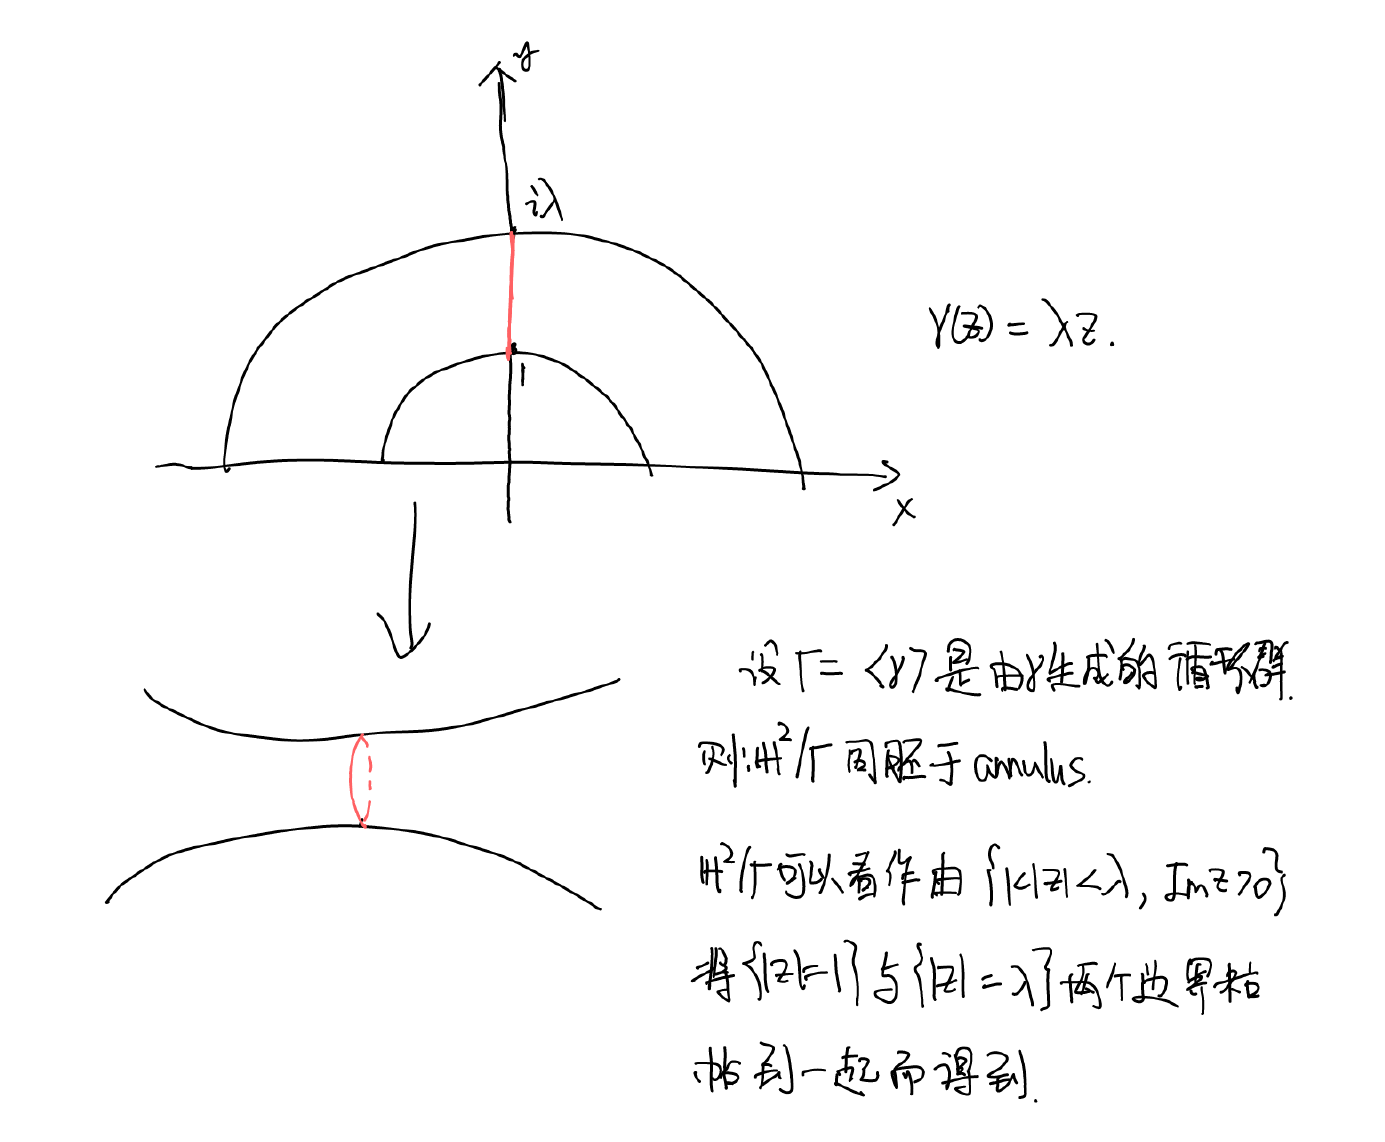
\includegraphics[scale=0.4]{images/hyperbolic_annulus.png}
    \caption{Hyperbolic Annulus}
    \label{hyperbolic_annulus}
\end{figure}

是$1-1$映射.  而$\lambda \cdot \{\abs{z}=1, \Im(z)>0\}= \{\abs{z}=\lambda, \Im(z)>0\}$. 因此, $\HH/\Gamma$可以由$\Omega_\lambda$将上下两边条边界粘贴在一起而得到. 见图\eqref{hyperbolic_annulus}. 而$\gamma$的轴投影到$\HH/\Gamma$上之后, 便成为一条闭测地线, 我们将这条闭测地线记为$\tilde{\gamma}$. 显然地, $\tilde{\gamma}$是$\pi_1(\HH/\Gamma)$的生成元. 而根据覆盖映射的性质, $\pi_1(\HH/\Gamma) = \Gamma= \left< \gamma \right>$.  因此, \textbf{$\gamma$可以自然地对应到$\tilde{\gamma}$, 后面我们将不再区分$\gamma$与$\tilde{\gamma}$}. 测地线$\tilde{\gamma}$的长度即为线段$\{\Re(z)=0, 1<\Im(z)< \lambda\}$的长度,

\begin{equation}
    l_{\tilde{\gamma}}= \int^\lambda_1 \frac{1}{y}dy=\log \lambda.
\end{equation}
我们也称$\log\lambda$为双曲型元素$\gamma$的长度.  $z \mapsto \lambda z$的矩阵表示为$\begin{pmatrix}
    &\sqrt{\lambda} \s 0 \\
    & 0 \s \rec{\sqrt{\lambda}}
\end{pmatrix}$. 于是有等式
\begin{equation}
    \begin{split}
        \text{Tr}(\begin{pmatrix}
                    &\sqrt{\lambda} \s 0 \\
                    & 0 \s \rec{\sqrt{\lambda}}
        \end{pmatrix}) = \sqrt{\lambda}+\rec{\sqrt{\lambda}} & = e^{\rec{\log \lambda}} + e^{-\rec{2}\log \lambda} \\ 
        & = 2\cosh(\frac{l_\gamma}{2}).
    \end{split}
\end{equation}
对于任意双曲型元素$\alpha \in \psl(2,\R)$, 由于$\gamma$可以共轭到$z \mapsto \lambda z$, 而在共轭作用下, 矩阵的迹是不变的.  则我们可以定义
\begin{equation}
    l_\alpha= 2\cosh^{-1}(\rec{2}\text{tr}(\alpha)).
\end{equation}
而$l_\alpha$即是$\alpha$的轴投影到曲面$\HH/\cycgroup{\alpha}$上后得到的闭测地线的长度.
\subsubsection{闭曲面上的双曲度量}
设$S_p$是亏格为$g\ge 2$的闭黎曼流形, 由等温坐标的存在性可知, $S_p$上可以赋予与黎曼度量相容的黎曼面结构. 而由单值化定理, $S_p$的万有覆盖空间同构于$\HH$(作为一个黎曼面). 由覆盖映射$\pi: \HH \to S_p$我们可以得到群嵌入$i: \pi_1(S_p) \hookrightarrow \psl(2,\R)$.  这样将$\pi_1(S_p)$看作$\psl(2,\R)$的子群后, 我们便得到了$S_p$上的双曲度量.
\begin{theorem}
    设$S_p$是亏格为$p \ge 2$的闭黎曼流形. 则在其黎曼度量的共形等价类中, 存在唯一的双曲度量.
\end{theorem}
\begin{definition}
    设$S_p$是亏格为$p$的光滑曲面.  设$G$是$S_p$上所有双曲度量的集合, 赋予$C^\infty$拓扑.  在$G$上定义等价关系$\sim$: 称$g_1, g_2 \in G$等价, 当且仅当存在等距同构$f: (S_p, g_1) \to (S_p, g_2)$, 即$df^*g_2=g_1$.  定义$\M_p=G/\sim$. 称$\M_p$为曲面$S_p$的模空间.
\end{definition}
\begin{theorem}
    $\M_g$是$6g-6$维的流形.
\end{theorem}
\begin{theorem}
    设$S_p$是亏格为$p$的光滑曲面. 设$\epsilon>0$. 设
    \begin{equation}
        \M_p^\epsilon=\{g \in \M_g\mid \text{对于任意简单闭曲线}\alpha \subset S_g, l_{\alpha,g} \ge \epsilon\}.
    \end{equation}
    则$\M_g$是紧的. 其中, $l_{\alpha,g}$表示曲线$\alpha$在度量$g$下的长度.
\end{theorem}
\par 设$S_{g,k}$是亏格为$g$, 有$k$个边界的黎曼面, 并且满足$2g+k-1 \ge 2$(这只排除了非常少的情况).
\chapter{黎曼流形中的Plateau问题}
\section{调和映射}
%\chapter{障碍问题}
\appendix
%\addcontentsline{toc}{chapter}{附录}
\chapter{附录}
\section{复分析基础}
%\section{等温坐标的存在性}
\begin{theorem}
    设$(\M^2, g)$是二维黎曼流形, 则存在$\M^2$上的一组坐标卡$\{z=x+iy\}$, 使得在这组坐标下, $g=\lambda^2\abs{dz}^2=\lambda^2(dx^2+dy^2)$, 并且这组坐标下的坐标变换是全纯的.
\end{theorem}
\begin{proof}
    固定点$p \in \M$. 取$p$点的足够小的邻域 $\Omega$, 在$\Omega$中, 取函数$u$ 使得
    \begin{equation}
        \Delta_g u= \Delta u + \Gamma^j_{ii}u_j=0.
    \end{equation}
    根据椭圆方程的理论, 这个方程总是局部可解的, 并且可以选取$u$使得$\nabla u(p) \ne 0$. 令$\omega= \sqrt{\det g}dx$为$\M$上的体积形式. 定义$1-$形式
    \begin{equation}
        \alpha= \Tr(\nabla u \otimes \omega)= i^*_{\nabla_u } \omega
    \end{equation}
    则 $d\alpha= \div(\nabla u)\omega =0$. 即, $\alpha$是闭的$1-$形式. 由Poincare引理可知, 存在函数$v$使得$\alpha= dv$.  现在,我们证明函数$u,v$具有如下关系:
    \begin{enumerate}
        \item $\inner{\nabla u}{\nabla v} =0$.
        \item $\abs{\nabla u}= \abs{\nabla v}$.
    \end{enumerate}
    对于性质(1), 我们有
    \begin{equation}
        \inner{\nabla u}{\nabla v} = dv(\nabla u) = \alpha(\nabla u)= (i^*_{\nabla u} w)\nabla u =0
    \end{equation}
    对于性质(2), 我们有
    \begin{equation}
        \inner{\nabla v}{\nabla v} = \inner{dv}{dv} = \inner{i^*_{\nabla u}\omega }{ i^*_{\nabla u}\omega}= \inner{\nabla u}{\nabla u}.
    \end{equation}
    上面的最后一个等式在测地坐标下是容易验证的. 
    \par 现在, 设$F(x,y)=(u,v)$. 在点$p$处, 由性质(1)可知, $\det dF(p) \ne 0$. 由反函数定理可知, $(u,v)$可以作为一组局部坐标. 在这组坐标下, 度量$g$的局部表示为
    \begin{equation}
        g=g_{uu}du^2+2g_{uv}dudv+g_{vv}dv^2
    \end{equation}
    由于
    \begin{align}
        &g_{uu}= \abs{\nabla u}^2 = \abs{\nabla v}^2= g_{vv} \\
        &g_{uv}=\inner{\nabla u}{\nabla v}=0. 
    \end{align}
    只需要取$z=u+iv$, $\lambda= \abs{\nabla u}$即可.
\end{proof}
%\section{调和共轭}
\begin{proposition}
    设$\Omega$是单连通区域. $u: \Omega \to \R$是调和函数. 则存在全纯函数$F$使得$u=\Re F$.
\end{proposition}
\begin{proof}
    由Riemann映射定理, 不妨设$\Omega = (0,1)\times (0,1)$或者 $\Omega= \mathbb{C}$.  定义
    \begin{equation}
        \tilde{v}(x,y)= \int^y_0 u_x(x,t)dt. 
    \end{equation}
    那么
    \begin{equation}
        \begin{split}
            \tilde{v}_x  =\int^y_0 u_{xx}(x,t)dt &=- \int^y_0 u_{tt}(x,t)dt \\
            &= -u_y(x,y)+u_y(x,0)
        \end{split}
    \end{equation}
    取$v(x,y)=\tilde{v}(x,y)- \int^x_0 u_y(t,0)dt$, 则$F(x,y)=u+iv$满足Cauchy-Riemann方程.
\end{proof}
\begin{theorem}[单值化定理]
    每一个单连通的黎曼曲面必定同构于$\mathbb{D}, \mathbb{C}, \mathbb{S}^2$中的三者之一.
\end{theorem}
%\section{黎曼几何基础}
%我们按照约定$\nabla^2_{X,Y}T=\nabla^2T(Y,X)$. 这样做是为了与欧氏空间的求导记号一致. 设$f\in C^\infty(\R^n)$, 则
%\begin{equation}
%    \nabla^2f(\PI,\PJ)=f_{ij}= \PJ \PI f = \nabla^2_{\PJ,\PI}f.
%\end{equation}
%\begin{remark}
%    总是先对离$f$近的记号求导.
%\end{remark}
%\begin{definition}
%    对于任意张量场$S$, 定义其曲率张量
%    \begin{equation}
%        R(X,Y)S=\nabla^2_{XY}S-\nabla^2_{YX}S
%    \end{equation}
%\end{definition}
%\begin{proposition}
%    设$f \in C^\infty(\M)$, 则
%    \begin{equation}
%        \nabla^3f(X,Y,Z)=\nabla^3f(X,Z,Y)+R(Z,Y,\nabla f, X)
%    \end{equation}
%\end{proposition}
%\begin{proof}
%    \begin{equation}
%        \begin{split}
%            \nabla^3f(X,Y,Z)-\nabla^3f(X,Z,Y) &=(\nabla^2_{Z,Y}\nabla f)(X)-(\nabla^2_{Y,Z}\nabla f)(X) \\
%            &= R(Z,Y,\nabla f, X)
%        \end{split}
%    \end{equation}
%\end{proof}
%%\addcontentsline{toc}{chapter}{附录}
\chapter{附录}
\section{复分析基础}
%\section{等温坐标的存在性}
\begin{theorem}
    设$(\M^2, g)$是二维黎曼流形, 则存在$\M^2$上的一组坐标卡$\{z=x+iy\}$, 使得在这组坐标下, $g=\lambda^2\abs{dz}^2=\lambda^2(dx^2+dy^2)$, 并且这组坐标下的坐标变换是全纯的.
\end{theorem}
\begin{proof}
    固定点$p \in \M$. 取$p$点的足够小的邻域 $\Omega$, 在$\Omega$中, 取函数$u$ 使得
    \begin{equation}
        \Delta_g u= \Delta u + \Gamma^j_{ii}u_j=0.
    \end{equation}
    根据椭圆方程的理论, 这个方程总是局部可解的, 并且可以选取$u$使得$\nabla u(p) \ne 0$. 令$\omega= \sqrt{\det g}dx$为$\M$上的体积形式. 定义$1-$形式
    \begin{equation}
        \alpha= \Tr(\nabla u \otimes \omega)= i^*_{\nabla_u } \omega
    \end{equation}
    则 $d\alpha= \div(\nabla u)\omega =0$. 即, $\alpha$是闭的$1-$形式. 由Poincare引理可知, 存在函数$v$使得$\alpha= dv$.  现在,我们证明函数$u,v$具有如下关系:
    \begin{enumerate}
        \item $\inner{\nabla u}{\nabla v} =0$.
        \item $\abs{\nabla u}= \abs{\nabla v}$.
    \end{enumerate}
    对于性质(1), 我们有
    \begin{equation}
        \inner{\nabla u}{\nabla v} = dv(\nabla u) = \alpha(\nabla u)= (i^*_{\nabla u} w)\nabla u =0
    \end{equation}
    对于性质(2), 我们有
    \begin{equation}
        \inner{\nabla v}{\nabla v} = \inner{dv}{dv} = \inner{i^*_{\nabla u}\omega }{ i^*_{\nabla u}\omega}= \inner{\nabla u}{\nabla u}.
    \end{equation}
    上面的最后一个等式在测地坐标下是容易验证的. 
    \par 现在, 设$F(x,y)=(u,v)$. 在点$p$处, 由性质(1)可知, $\det dF(p) \ne 0$. 由反函数定理可知, $(u,v)$可以作为一组局部坐标. 在这组坐标下, 度量$g$的局部表示为
    \begin{equation}
        g=g_{uu}du^2+2g_{uv}dudv+g_{vv}dv^2
    \end{equation}
    由于
    \begin{align}
        &g_{uu}= \abs{\nabla u}^2 = \abs{\nabla v}^2= g_{vv} \\
        &g_{uv}=\inner{\nabla u}{\nabla v}=0. 
    \end{align}
    只需要取$z=u+iv$, $\lambda= \abs{\nabla u}$即可.
\end{proof}
%\section{调和共轭}
\begin{proposition}
    设$\Omega$是单连通区域. $u: \Omega \to \R$是调和函数. 则存在全纯函数$F$使得$u=\Re F$.
\end{proposition}
\begin{proof}
    由Riemann映射定理, 不妨设$\Omega = (0,1)\times (0,1)$或者 $\Omega= \mathbb{C}$.  定义
    \begin{equation}
        \tilde{v}(x,y)= \int^y_0 u_x(x,t)dt. 
    \end{equation}
    那么
    \begin{equation}
        \begin{split}
            \tilde{v}_x  =\int^y_0 u_{xx}(x,t)dt &=- \int^y_0 u_{tt}(x,t)dt \\
            &= -u_y(x,y)+u_y(x,0)
        \end{split}
    \end{equation}
    取$v(x,y)=\tilde{v}(x,y)- \int^x_0 u_y(t,0)dt$, 则$F(x,y)=u+iv$满足Cauchy-Riemann方程.
\end{proof}
\begin{theorem}[单值化定理]
    每一个单连通的黎曼曲面必定同构于$\mathbb{D}, \mathbb{C}, \mathbb{S}^2$中的三者之一.
\end{theorem}
%\section{黎曼几何基础}
%我们按照约定$\nabla^2_{X,Y}T=\nabla^2T(Y,X)$. 这样做是为了与欧氏空间的求导记号一致. 设$f\in C^\infty(\R^n)$, 则
%\begin{equation}
%    \nabla^2f(\PI,\PJ)=f_{ij}= \PJ \PI f = \nabla^2_{\PJ,\PI}f.
%\end{equation}
%\begin{remark}
%    总是先对离$f$近的记号求导.
%\end{remark}
%\begin{definition}
%    对于任意张量场$S$, 定义其曲率张量
%    \begin{equation}
%        R(X,Y)S=\nabla^2_{XY}S-\nabla^2_{YX}S
%    \end{equation}
%\end{definition}
%\begin{proposition}
%    设$f \in C^\infty(\M)$, 则
%    \begin{equation}
%        \nabla^3f(X,Y,Z)=\nabla^3f(X,Z,Y)+R(Z,Y,\nabla f, X)
%    \end{equation}
%\end{proposition}
%\begin{proof}
%    \begin{equation}
%        \begin{split}
%            \nabla^3f(X,Y,Z)-\nabla^3f(X,Z,Y) &=(\nabla^2_{Z,Y}\nabla f)(X)-(\nabla^2_{Y,Z}\nabla f)(X) \\
%            &= R(Z,Y,\nabla f, X)
%        \end{split}
%    \end{equation}
%\end{proof}
%\section{PDE基础}
%\appendix
\chapter{习题}
\begin{enumerate}
    \item 设$\Omega\subset \R^n$是有界区域. 设$u \in W^{1,1}(\Omega)$.  设$\Area(u)=\int_\Omega \sqrt{1+\abs{Du}^2}$. 证明: $\Area(u)$在$W^{1,1}(\Omega)$上是严格凸的.
    \item 证明: $\R^n$中不存在紧致无边的极小曲面.
    \item 设 $\Sigma \subset \R^3$是极小曲面. 设存在平面$P$使得$\Sigma \perp P$. 设$\Sigma$关于平面$P$的反射后的像为$\Sigma'$. 证明: $\Sigma \cup \Sigma'$是极小曲面.
    \item 设$f: \Omega \to \mathbb{C}$是光滑函数. 证明:
    \begin{enumerate}
        \item $f$全纯当且仅当 $\barpartial f=0$.
        \item $f$调和当且仅当$\partial \barpartial f=0$.
    \end{enumerate}
    \item 设$\Sigma$为Catenoid. $\Gamma_a=\Sigma \cap \{z=\pm a\}$. 试比较以下三个以$\Gamma_a$为边界的曲面的面积大小.
    \begin{enumerate}
        \item $\Gamma_a$所围的两个圆盘之并.  
        \begin{equation*}
            \Sigma_1=\{(x,y,z)\mid \sqrt{x^2+y^2} \le \cosh a, z=\pm a\}.
        \end{equation*}
        \item $\Gamma_a$的两个分支之间的柱面. 
        \begin{equation*}
            \Sigma_2=\{(x,y,z)\mid \sqrt{x^2+y^2} = \cosh a, \abs{z} \le a\}.
        \end{equation*}
        \item $\Gamma_a$之间Catenoid的部分. 
        \begin{equation*}
            \Sigma_3=\{(x,y,z)\mid  \sqrt{x^2+y^2}=\cosh z, \abs{z} \le a \}.
        \end{equation*}
    \end{enumerate}
    \item 设$\gamma\subset \R^3$是 $xz$平面上的曲线. $\gamma= \{(x,0,z)\mid x=f(z) >0 \}$. 由$\gamma$ 绕$z$轴旋转所得到的曲面记为$\Sigma$. 若$\Sigma$是极小曲面, 试求$f$的表达式.
    \item 设$\Sigma^{n-1} \subset \M^n$是极小曲面. $F(x,t): \Sigma \times (-\epsilon, \epsilon)\to \M$是固定边界的变分. 设$H_t$为 $\Sigma_t$的平均曲率. 计算 $\ddt H_t \mid _{t=0}$.
    \item 设$u$是Catenoid上的有界调和函数, 证明$u$是常数.
    \item 设$\M^3$可定向且$\Sigma^2 \subset \M^3$是定向的稳定极小曲面. 设$\tilde{\Sigma}$是$\Sigma$的覆盖空间. 则覆盖映射$f:\tilde{\Sigma}\to \Sigma \hookrightarrow \M$是稳定极小曲面.
    \item 设$\Sigma^{n-1} \subset \M^n$是极小曲面. 证明: $\forall p \in \Sigma$, 存在$p$点的足够小的邻域$\Omega$使得$\Omega \cap \Sigma$是稳定的.
\end{enumerate}
%\nocite{*}
%\clearpage
%%\phantomsection
%%\addcontentsline{toc}{section}{参考文献}
\tolerance=500
\printbibliography[heading=bibintoc, title=参考文献]
\end{document}